\documentclass[aspectratio=169]{beamer} % Formato widescreen per il diagramma a blocchi

% --- IMPOSTAZIONI TEMA ---
\usetheme{Madrid}
\usecolortheme{whale}
\setbeamertemplate{navigation symbols}{} % Rimuove i simboli di navigazione in basso
\setbeamertemplate{caption}[numbered]

% --- PACCHETTI STANDARD ---
\usepackage[utf8]{inputenc}
\usepackage[T1]{fontenc}
\usepackage[italian]{babel}
\usepackage{lmodern} % RISOLVE IL WARNING SUI FONT BOLD
\usepackage{amsmath, amsfonts, amssymb}
\usepackage{booktabs} % Per tabelle più belle
\usepackage{caption}
\usepackage{subcaption}
\usepackage{bm}
\usepackage{siunitx}
\usepackage{colortbl}
\usepackage{pifont}
% --- PACCHETTI PER GRAFICA E SCHEMI (TIKZ) ---
\usepackage{tikz}
\usetikzlibrary{shapes.geometric, arrows.meta, fit, calc, positioning, backgrounds}


\usepackage{graphicx}
\graphicspath{{../../img/}{../../img/controllo_verticale/}}
\renewcommand{\figurename}{Fig.}

% --- METADATI ---
\title{Modellazione dinamica e design del controllo per un innovativo VTOL}
\author{Maria Costanza Giacona}
\date{}

\begin{document}

% --- SLIDE TITOLO ---
\begin{frame}
    \titlepage
    \vfill
    \large
    \begin{center}
        Università degli Studi di Roma Tor Vergata\\
        \vspace{0.2cm}
        Dipartimento di Ingegneria
    \end{center}
    \vfill
\end{frame}

% --- INDICE ---
\begin{frame}{Sommario}
    \tableofcontents
\end{frame}

% ============================================================
% PARTE 0: INTRODUZIONE
% ============================================================
\section{Introduzione}

\begin{frame}
    \vfill
    \centering
    {\Huge \textbf{Introduzione}}
    \vfill
\end{frame}

\begin{frame}{Introduzione}
    L'interesse per gli UAV è in forte crescita (sorveglianza, agricoltura, ricerca e soccorso).
    Tuttavia, le configurazioni classiche presentano limitazioni:

    \vspace{0.2cm}
   \begin{columns}[t]
        \column{0.48\textwidth}
        \textbf{Multirotori}
        \begin{itemize}
            % NOTA: Le parentesi graffe { } extra servono a proteggere il comando nel beamer
            \item[{\textcolor{green}{\checkmark}}] Semplicità, Hovering stabile.
            \item[{\textcolor{red}{$\times$}}] Bassa efficienza, Range ridotto.
        \end{itemize}
        \centering
        \begin{figure}
            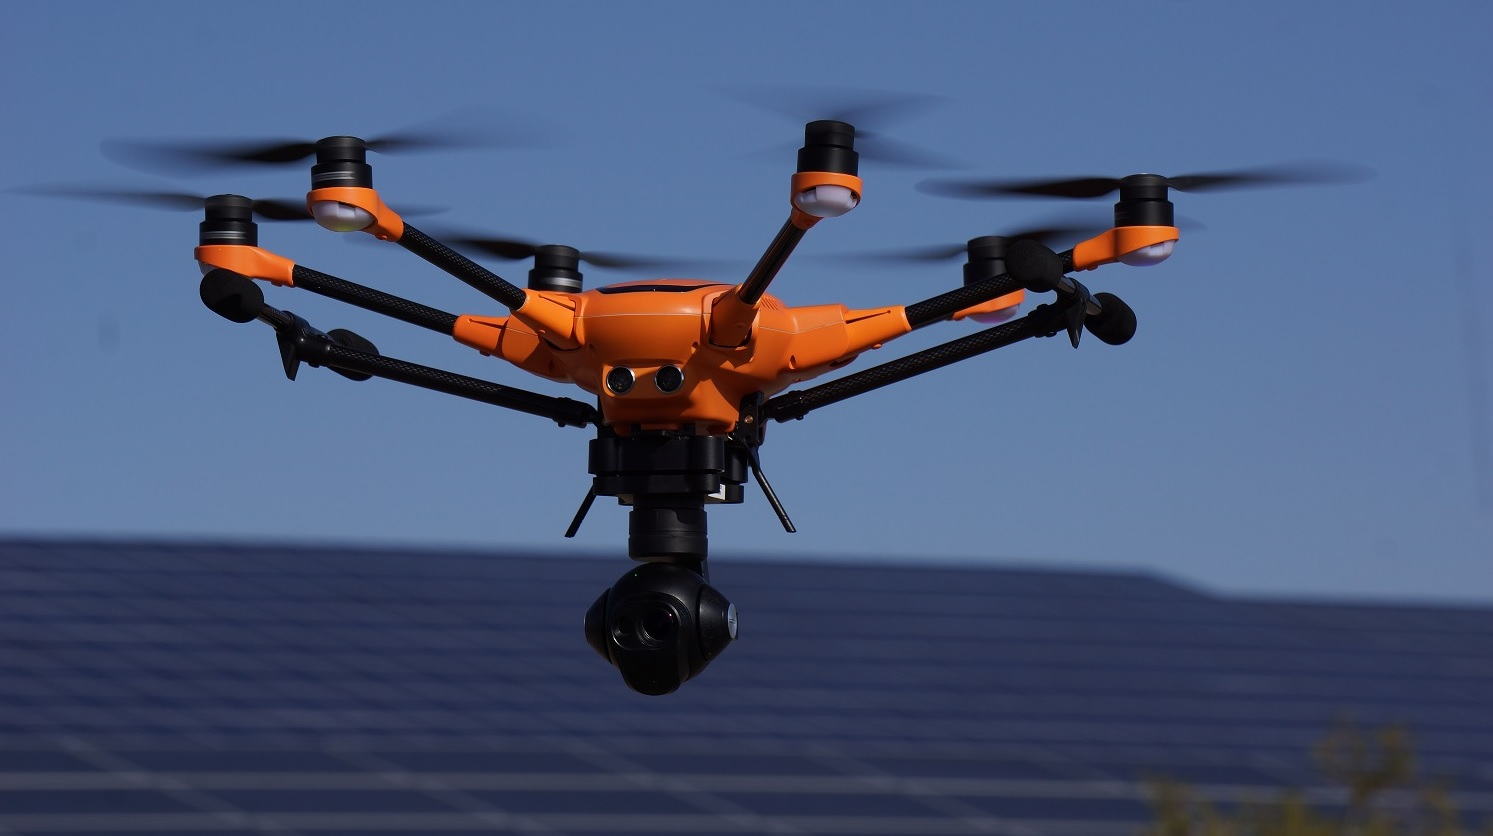
\includegraphics[width=0.6\textwidth]{multicopter.png}
            \caption{multicottero}
        \end{figure} 
        
        \column{0.48\textwidth}
        \textbf{Ala Fissa}
        \begin{itemize}
            \item[{\textcolor{green}{\checkmark}}] Alta efficienza, Lungo raggio.
            \item[{\textcolor{red}{$\times$}}] Necessità piste, No hovering.
        \end{itemize}
        \centering
        \begin{figure}
            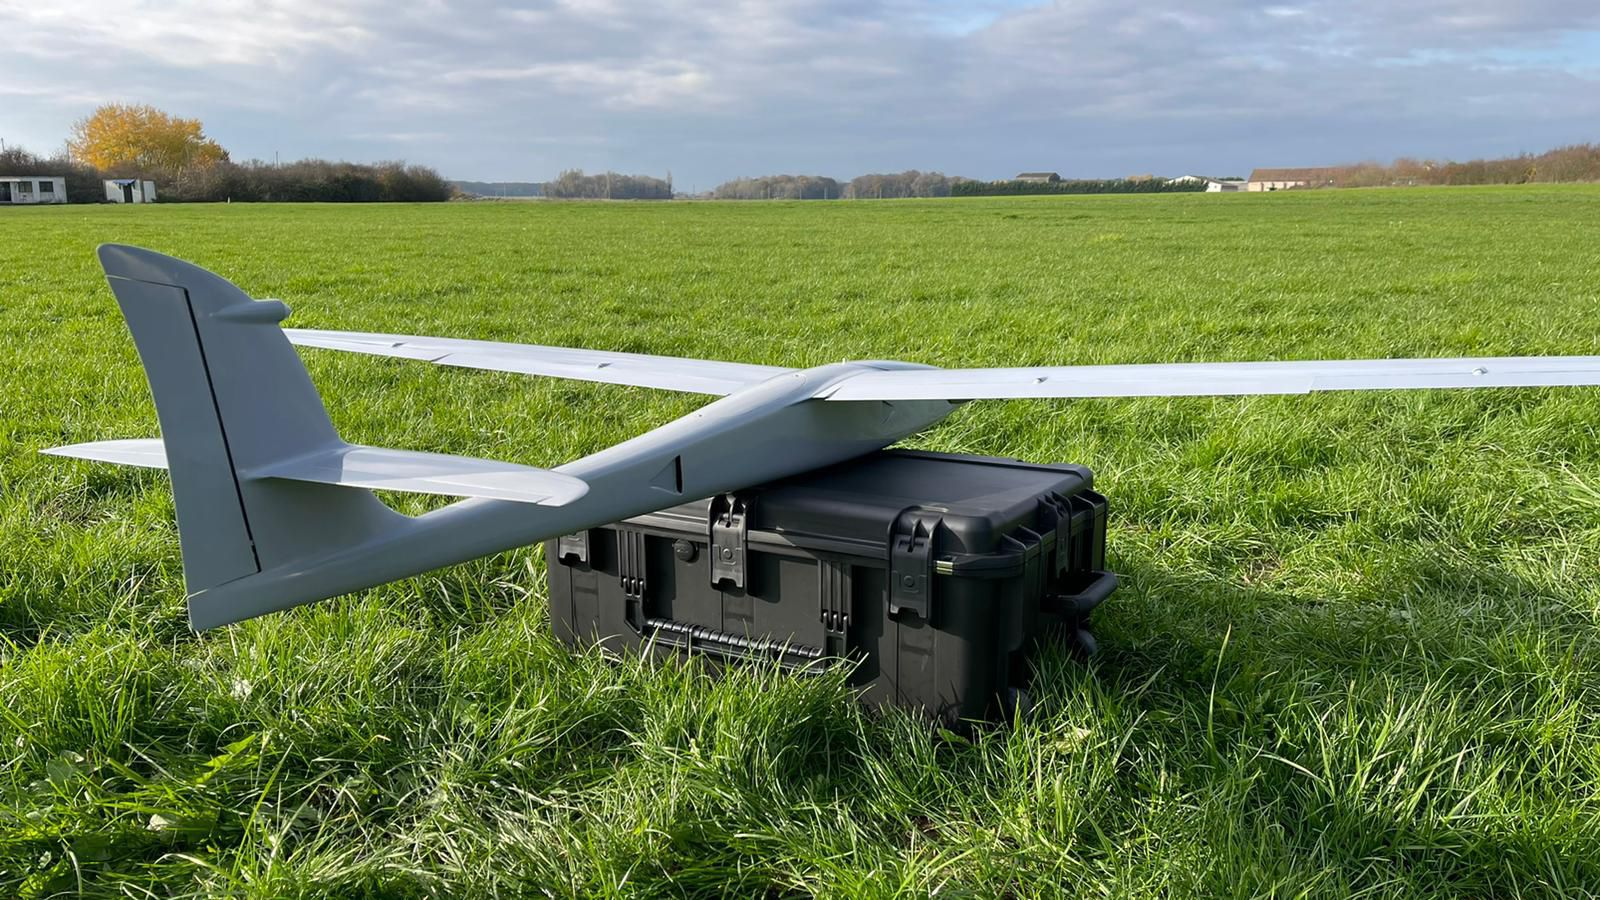
\includegraphics[width=0.6\textwidth]{fixed_wing.png}
            \caption{aereo}
        \end{figure}       
    \end{columns}

    % \vspace{0.2cm}
    \centering
    \textbf{Soluzione:} Configurazione Ibrida (VTOL)
\end{frame}

\section{Descrizione VTOL}

\begin{frame}
    \vfill
    \centering
    {\Huge \textbf{Descrizione VTOL}}
    \vfill
\end{frame}

\begin{frame}{VTOL tilting-rotor}
    Il tricottero \textit{tilting-rotor} combina i benefici delle due architetture:
    
    \begin{columns}
        \column{0.6\textwidth}
        \begin{itemize}
            \item \textbf{Decollo/Atterraggio:} Verticale (come un elicottero), indipendente da infrastrutture.
            \item \textbf{Crociera:} Volo aerodinamico (come un aereo) ruotando i propulsori.
        \end{itemize}
        
        \vspace{0.5cm}
        \begin{block}{La Sfida Ingegneristica}
            Questa versatilità introduce una \textbf{dinamica complessa} e fortemente accoppiata, 
            richiedendo strategie di controllo avanzate.
        \end{block}

        \column{0.4\textwidth}
        \centering
        \begin{figure}
            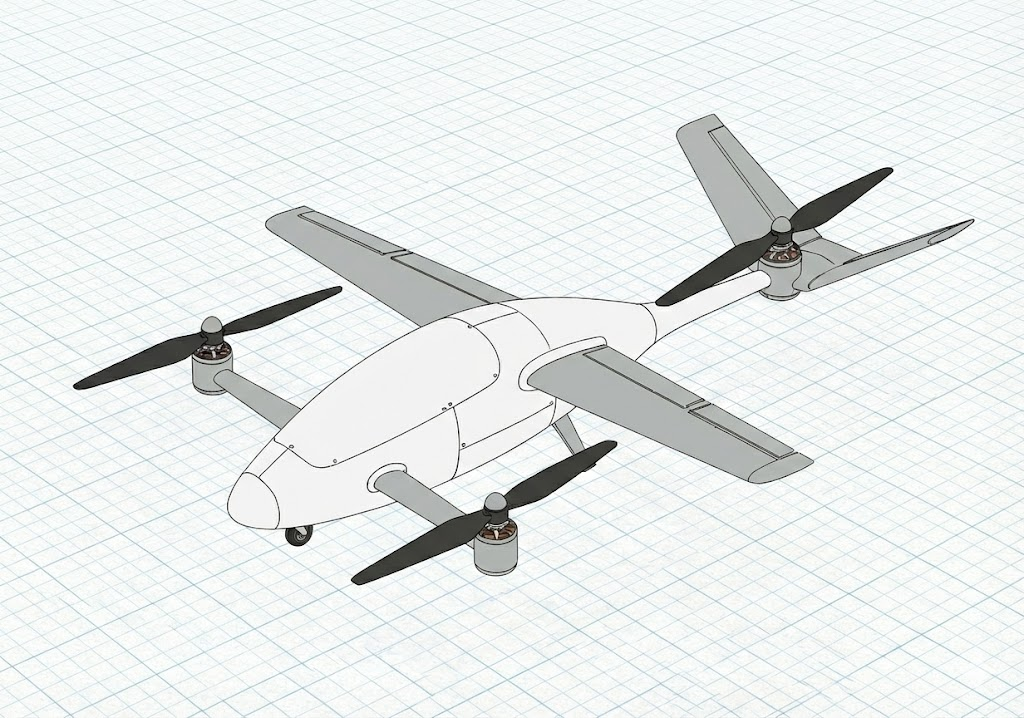
\includegraphics[width=0.8\textwidth]{VTOL.png}
            \caption{\footnotesize Rendering del velivolo.}
        \end{figure}
        
    \end{columns}
\end{frame}

\begin{frame}{Tricottero tilting-rotor}
    \begin{columns}[c] % [c] centra verticalmente il contenuto delle colonne
        \column{0.55\textwidth}
        Nello specifico, il tricottero in esame presenta i rotori orientabili, ma non ha superfici geometriche variabili.
        
        \vspace{0.5cm} % Un po' di respiro tra i paragrafi
        Questa configurazione rappresenta una criticità in fase di crociera perché è necessario gestire sia assetto che posizione solo tramite la vettorizzazione della spinta.

        \column{0.45\textwidth}
        \begin{figure}
            \centering
            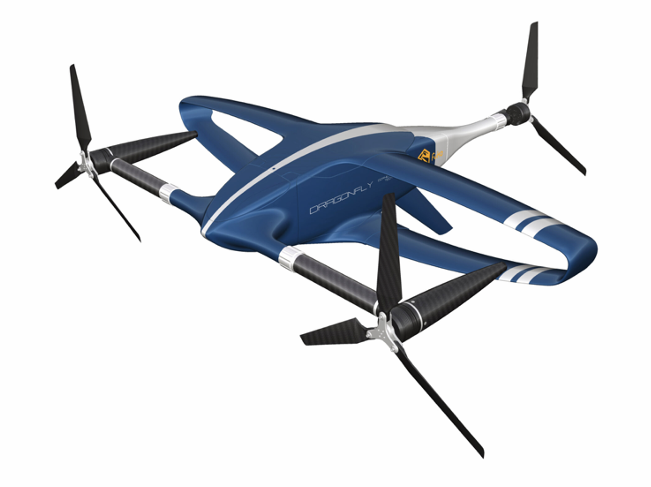
\includegraphics[width=\columnwidth]{dragonfly.png} 
            \caption{Dragonfly.}
        \end{figure}
    \end{columns}
\end{frame}

% ============================================================
% 2. MODELLAZIONE (RIELABORATA)
% ============================================================
\section{Modello Matematico}

\begin{frame}
    \vfill
    \centering
    {\Huge \textbf{Modello Matematico}}
    \vfill
\end{frame}

% --- SLIDE 1: SISTEMI DI RIFERIMENTO ---
% Mantenuta simile, pulita la formattazione
\begin{frame}{Sistemi di Riferimento}
    \small
    Per descrivere la dinamica 6-DOF si adottano due sistemi destrorsi:
    \vspace{-0.5cm}
    \begin{columns}[t]
        \begin{column}{0.5\textwidth}
            \begin{itemize}
                \item \textbf{Inerziale ($\mathcal{F}_g$):} \\
                Posizione $\bm{P}_g$, Assetto $\bm{\Theta}_g$ (Eulero).
                \begin{center}
                    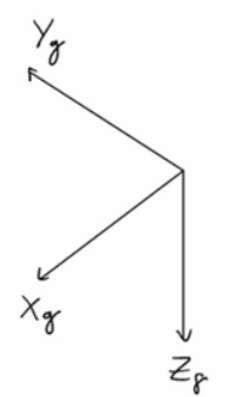
\includegraphics[height=3cm]{sist_rif_global.png}
                    \captionof{figure}{Sistema inerziale.}
                \end{center}
            \end{itemize}
        \end{column}
        \begin{column}{0.5\textwidth}
            \begin{itemize}
                \item \textbf{Solidale ($\mathcal{F}_b$):} 
                    Origine nel \textbf{CoM}. \\
                    Velocità $\bm{V}_b = [u, v, w]^T$, $\bm{\Omega}_b = [p, q, r]^T$.
                    \begin{center}
                        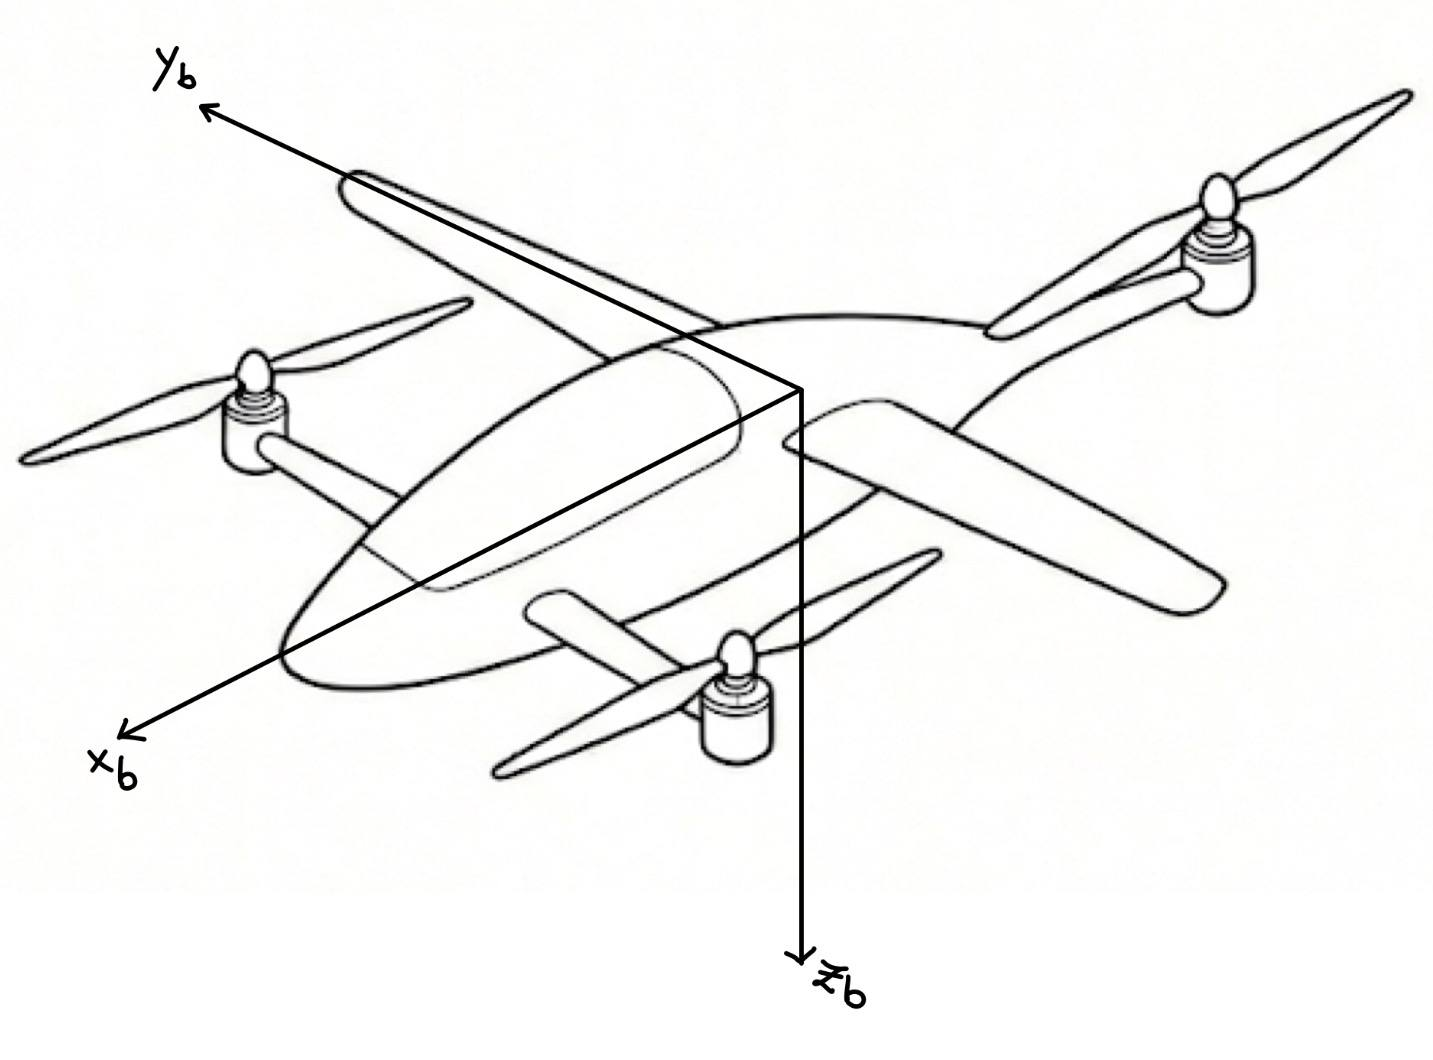
\includegraphics[height=3cm]{sist_rif_body.jpg}
                        \captionof{figure}{Sistema solidale al corpo.}
                    \end{center}
            \end{itemize}
        \end{column}
    \end{columns}
    
    \vspace{0.1cm}
    \textbf{Cinematica (Relazione tra i sistemi):}
    \begin{equation}
        \begin{bmatrix} \bm{\dot{P}}_g \\ \bm{\dot{\Theta}}_g \end{bmatrix} = 
        \begin{bmatrix} \mathbf{R}_{b \to g}(\bm{\Theta}) & \mathbf{0} \\ \mathbf{0} & \mathbf{J}_{b \to g}(\bm{\Theta}) \end{bmatrix}
        \begin{bmatrix} \bm{V}_b \\ \bm{\Omega}_b \end{bmatrix}
    \end{equation}
\end{frame}

% --- SLIDE 2: CONFIGURAZIONE E PROBLEMA ---
% Focus sull'accoppiamento geometrico
\begin{frame}{Configurazione Geometrica e Attuazione}
    \begin{columns}[c]
        \begin{column}{0.5\textwidth}
            \centering
            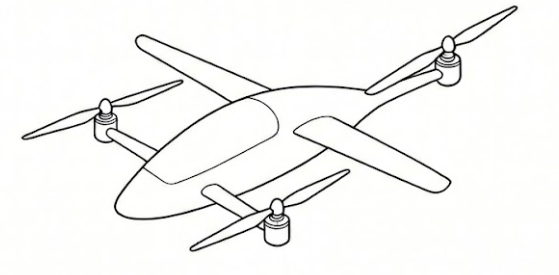
\includegraphics[width=0.9\linewidth]{tricopter_2D.png}
            \captionof{figure}{Configurazione rotori avanzati ($d_x > 0$).}
        \end{column}
        
        \begin{column}{0.5\textwidth}
            \textbf{Configurazione:}
            \begin{itemize}
                \item Rotori Anteriori: $\bm{r}_{1,2} = [d_{mx}, \pm d_{my}, 0]^T$
                \item Rotore di Coda: $\bm{r}_3 = [-d_{tx}, 0, 0]^T$
            \end{itemize}
            
            \vspace{0.5cm}
            \begin{alertblock}{Criticità Dinamica}
                La spinta totale non è applicata nel CoM. 
                \textbf{Implicazione:} Il bilanciamento del \textit{Pitch} richiede una ripartizione di potenza asimmetrica tra rotori anteriori e posteriore.
            \end{alertblock}
        \end{column}
    \end{columns}
\end{frame}

\begin{frame}{Configurazione dei rotori}
    Il tricottero dispone di 3 motori con gradi di libertà di tilt:
    
    \vspace{0.5cm}
    \begin{columns}
        \column{0.5\textwidth}
        \centering
        \textbf{Rotori Anteriori}
        % SOSTITUISCI CON 'rotori_1_2.png'
        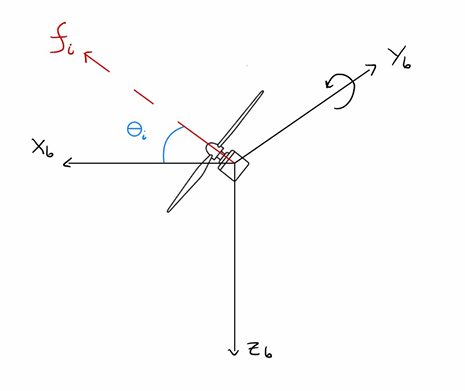
\includegraphics[width=0.7\textwidth]{rotori_1_2.png}
        \vspace{0.2cm}\\
        \footnotesize{Tilt attorno all'asse $Y_b$.}
        
        \column{0.5\textwidth}
        \centering
        \textbf{Rotore di Coda}
        % SOSTITUISCI CON 'rotore_3.png'
        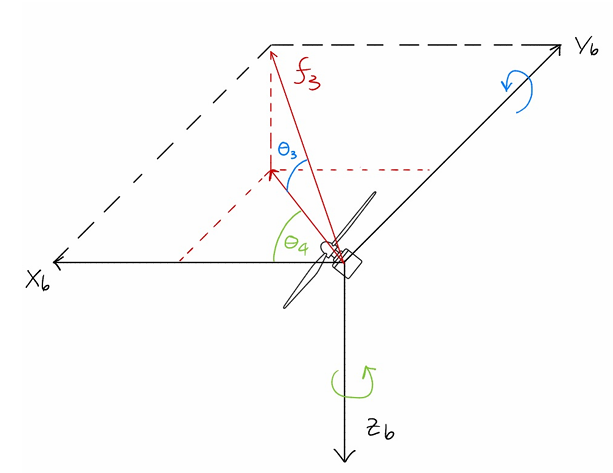
\includegraphics[width=0.7\textwidth]{rotore_3.png}
        \vspace{0.25cm}\\
        \footnotesize{Tilt su $Y_b$ e $Z_b$.}
    \end{columns}
    
\end{frame}

% --- SLIDE 3: NEWTON-EULERO ---
% Forma vettoriale compatta, molto più elegante
\begin{frame}{Equazioni della Dinamica: Newton-Eulero}
    Il modello del corpo rigido è descritto dalle equazioni cardinali nel \textit{Body Frame}:
    
    \vspace{0.5cm}
    \begin{block}{Dinamica Traslazionale e Rotazionale}
    \begin{equation}
        \begin{cases}
            m \bm{\dot{V}}_b = \bm{F}_{\text{tot}} - \underbrace{\bm{\Omega}_b \times (m \bm{V}_b)}_{\text{Coriolis}} \\
            \mathbf{I}_b \bm{\dot{\Omega}}_b = \bm{M}_{\text{tot}} - \underbrace{\bm{\Omega}_b \times (\mathbf{I}_b \bm{\Omega}_b)}_{\text{Giroscopico Body}}
        \end{cases}
    \end{equation}
    \end{block}
    
    \vspace{0.5cm}
    \textbf{Scomposizione delle Forze e Momenti:}
    \begin{itemize}
        \item $\bm{F}_{\text{tot}} = \bm{F}_{\text{th}} + \bm{F}_g + \bm{F}_{\text{aero}}$
        \item $\bm{M}_{\text{tot}} = \bm{M}_{\text{th}} + \bm{M}_{\text{tor}} + \bm{M}_{\text{aero}} + \bm{M}_{\text{gyro}} + \bm{M}_{\text{pinna}}$
    \end{itemize}
\end{frame}

% --- SLIDE 4: FORZE ESTERNE ---
% Condensata: Spinta e Aerodinamica insieme
\begin{frame}{Analisi delle Forze}
    \begin{columns}[T]
        \begin{column}{0.5\textwidth}
            \textbf{1. Spinta Motori ($\bm{F}_{th}$)} \\
            Dipende dall'orientamento ($\theta_i$) e velocità ($\omega_i$) dei rotori:
            \begin{equation*}
                \bm{F}_{th} = \sum_{i=1}^3 \mathbf{R}_{rot_i \to b}(\theta_i) \cdot [0, 0, k\omega_i^2]^T
            \end{equation*}
            
            \vspace{0.2cm}
            \textbf{2. Gravità ($\bm{F}_g$)} \\
            Proiezione del vettore peso nel body frame:
            \begin{equation*}
                \bm{F}_g = \mathbf{R}_{g \to b} \cdot [0, 0, mg]^T
            \end{equation*}
        \end{column}
        
        \begin{column}{0.5\textwidth}
            \textbf{3. Aerodinamica ($\bm{F}_{aero}$)} \\
            Modello non-lineare per fusoliera e ali:
            \begin{equation*}
                \bm{F}_{wing} \propto \frac{1}{2}\rho S v^2 \cdot \begin{bmatrix} C_D(\alpha) \\ 0 \\ C_L(\alpha) \end{bmatrix}
            \end{equation*}
            \vspace{0.1cm}
            \centering
            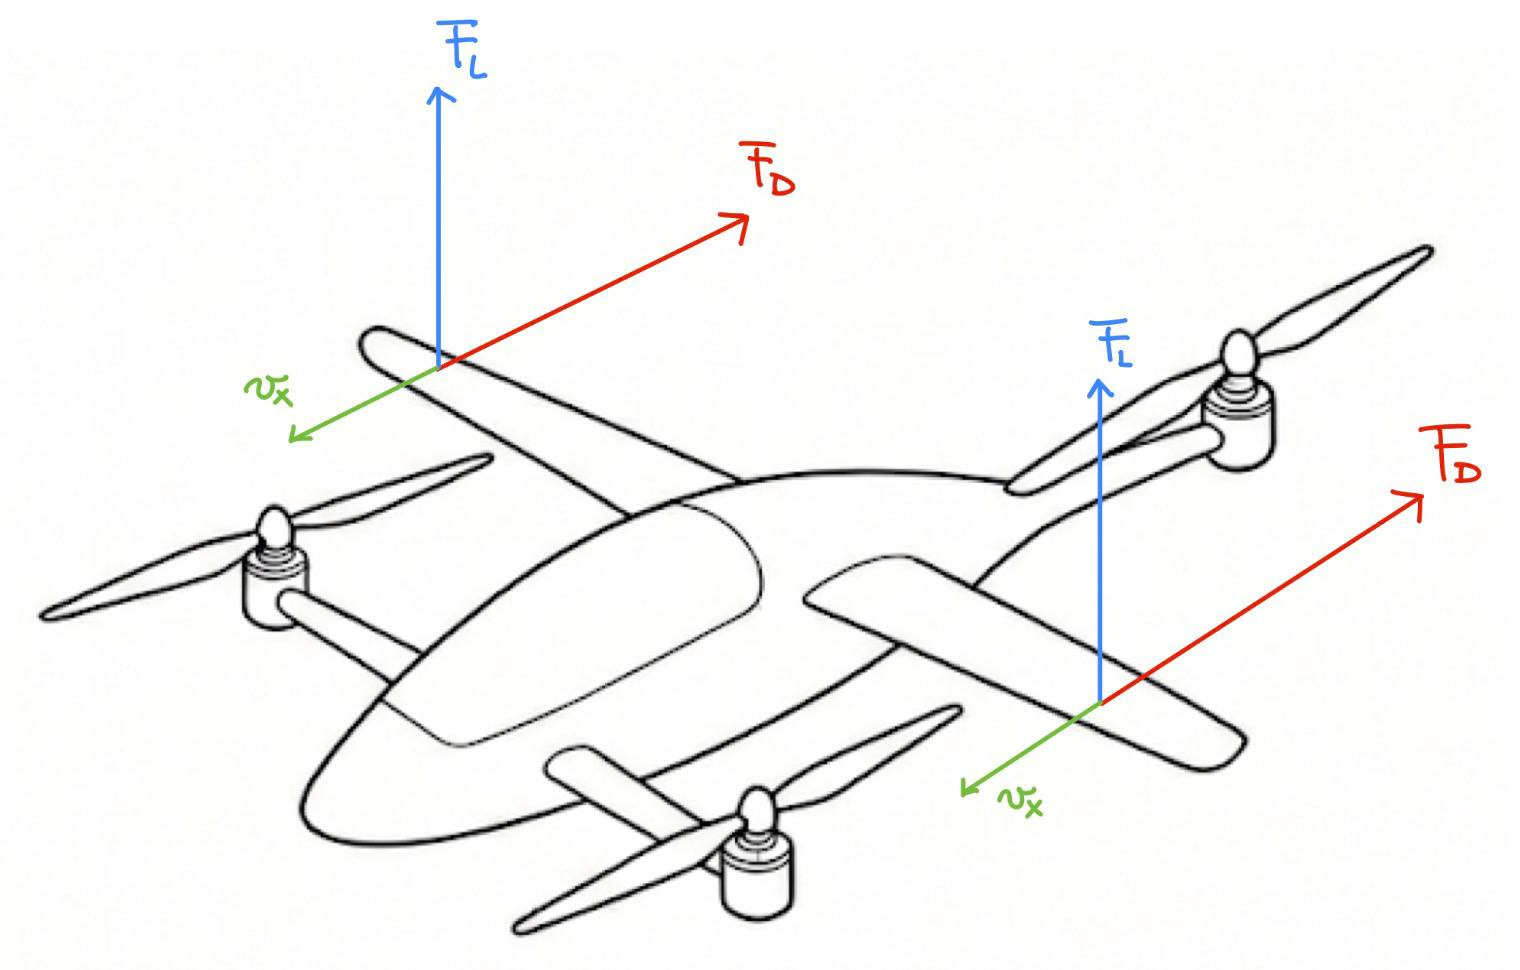
\includegraphics[width=0.68\linewidth]{forze_x.jpg}
            \captionof{figure}{Drag e Lift.}
        \end{column}
    \end{columns}
\end{frame}

% --- SLIDE 5: MOMENTI ATTIVI (Thrust & Torque) ---
% Raggruppa le slide 16 e 17 originali
\begin{frame}{Momenti Attivi: Controllo del Velivolo}
    I momenti di controllo sono generati dalla combinazione di spinta e reazione dei rotori.
    
    \vspace{0.3cm}
    \textbf{1. Momento di Spinta ($\bm{M}_{th}$)}
    \begin{equation}
        \bm{M}_{\text{th}} = \sum_{i=1}^{3} (\bm{r}_i \times \bm{F}_{th_{i}})
    \end{equation}

    \vspace{0.4cm}
    \textbf{2. Momento Torcente ($\bm{M}_{tor}$)}
    \begin{equation}
        \bm{M}_{\text{tor}} = \sum_{i=1}^{3} (b \omega_i^2 + I_{rot} \dot{\omega}_i) \hat{e}_{thrust,i}
    \end{equation}
\end{frame}

% --- SLIDE 6: MOMENTI REATTIVI (Giroscopico & Pinna) ---
% Raggruppa le slide 19, 20, 21 originali. 
% ELIMINATA la matrice gigante del giroscopico tilting a favore della forma vettoriale.
\begin{frame}{Momenti Reattivi e Dinamica Veloce}
    Effetti dinamici dovuti alla rotazione dei componenti e alla stabilizzazione passiva.

    \begin{block}{Effetto Giroscopico dei Rotori (Tilting)}
        Nasce dall'inclinazione dei rotori in azione ($\bm{\omega}_{tilt}$):
        \begin{equation}
             \bm{M}_{\text{giro}} = \sum_{i=1}^{3} \mathbf{J}_{r} (\bm{\omega}_{\text{tilt},i} \times \bm{\omega}_{r,i})
        \end{equation}
    \end{block}

    \vspace{0.3cm}
    \begin{columns}[t]
        \begin{column}{0.5\textwidth}
            \textbf{Momento Pinna di Coda:}
            \begin{equation*}
                M_{z, pinna} \propto -r \cdot v_y^2
            \end{equation*}
            Smorzamento naturale sull'asse di imbardata.
        \end{column}
        \begin{column}{0.5\textwidth}
             \textbf{Giroscopico Body:}
             \begin{equation*}
                 \bm{\Omega}_b \times (\mathbf{I}_b \bm{\Omega}_b)
             \end{equation*}
             Momento giroscopisco dovuto alla rotazione del velivolo nel \textit{body frame}.
        \end{column}
    \end{columns}
\end{frame}

% ==========================================================
% 3. SISTEMA DINAMICO (RIELABORATO)
% ==========================================================
\section{Sistema Dinamico}

\begin{frame}
    \vfill
    \centering
    {\Huge \textbf{Sistema Dinamico}}
    \vfill
\end{frame}

% --- SLIDE 1: FORMULAZIONE DELLO STATO ---
% Unisce definizione e variabili in una sola visione d'insieme potente
\begin{frame}{Formulazione nello Spazio di Stato}
    Il modello è tradotto in un sistema di ODE del tipo $\dot{\mathbf{x}} = f(\mathbf{x}, \mathbf{u}, t)$.
    
    \vspace{0.5cm}
    \textbf{Vettore di Stato ($\mathbf{x} \in \mathbb{R}^{26}$):}
    \begin{equation}
        \mathbf{x} = 
        {
            \renewcommand{\arraystretch}{1.2}
        \begin{bmatrix}
            \bm{P}_g \\ \bm{V}_b \\ \hline
            \bm{\Theta}_g \\ \bm{\Omega}_b \\ \hline
            \bm{\theta}_{rot} \\ \bm{\dot{\theta}}_{rot} \\ \hline
            \bm{\omega}_{rot} \\ \bm{\dot{\omega}}_{rot}
        \end{bmatrix}
        }
        \begin{array}{l}
            \left. \begin{matrix} \text{Posizione Inerziale } [x,y,z] \\ \text{Velocità Body } [u,v,w] \end{matrix} \right\} \text{\textbf{Traslazione}} \\[1em]
            \left. \begin{matrix} \text{Assetto Eulero } [\phi,\theta,\psi] \\ \text{Velocità Angolari } [p,q,r] \end{matrix} \right\} \text{\textbf{Rotazione}} \\[1em]
            \left. \begin{matrix} \text{Posizione Servi} \\ \text{Velocità Servi} \end{matrix} \right\} \text{\textbf{Dinamica Servi}} \\[1em]
            \left. \begin{matrix} \text{Velocità Rotori} \\ \text{Accel. Rotori} \end{matrix} \right\} \text{\textbf{Propulsione}}
        \end{array}
    \end{equation}
\end{frame}

% --- SLIDE 2: INGRESSI DI CONTROLLO ---
% Più pulita, usa colonne per separare logica e matematica
\begin{frame}{Ingressi di Controllo ($\mathbf{u} \in \mathbb{R}^7$)}
    Il vettore degli ingressi $\mathbf{u}$ gestisce sia la potenza che la geometria del velivolo.

    \vspace{0.5cm}
    \begin{columns}[c]
        \begin{column}{0.4\textwidth}
            \centering
            \begin{equation*}
                \mathbf{u} = \begin{bmatrix} 
                u_1 \\ u_2 \\ u_3 \\ \hline
                u_4 \\ u_5 \\ \hline
                u_6 \\ u_7 
                \end{bmatrix}
            \end{equation*}
        \end{column}

        \begin{column}{0.6\textwidth}
            \begin{itemize}
                \item[] \textbf{Propulsione}
                \begin{itemize}
                    \item[$u_{1-3}$:] Velocità angolari per i tre motori.
                \end{itemize}
                \vspace{0.3cm}
                \item[] \textbf{Tilt Anteriore}
                \begin{itemize}
                    \item[$u_{4,5}$:] Angoli di tilt per rotori anteriori.
                \end{itemize}
                \vspace{0.3cm}
                \item[] \textbf{Tilt Coda}
                \begin{itemize}
                    \item[$u_{6,7}$:] Angoli di tilt rotore di coda.
                \end{itemize}
            \end{itemize}
        \end{column}
    \end{columns}
\end{frame}

% --- SLIDE 3: DINAMICA ATTUATORI ---
% Questa è la slide critica. Sostituisce la cinematica standard con la dinamica realistica
\begin{frame}{Dinamica degli Attuatori}
    La modellazione include la dinamica del \textbf{secondo ordine} per distinguere la risposta fisica dei servomotori e dei motori dei rotori.

    \begin{columns}[t]
        \begin{column}{0.48\textwidth}
            \begin{block}{Servomotori di Tilting}
            Gestiscono l'orientamento dei rotori ($x_{13} \dots x_{20}$):
            \begin{equation*}
                \begin{cases} 
                \dot{x}_{i} = x_{i+1} \\ 
                \dot{x}_{i+1} = -2\zeta_j \omega_{n,j} x_{i+1} + \omega_{n,j}^2 (u_k - x_i)
                \end{cases}
            \end{equation*}
            \end{block}
        \end{column}
        \begin{column}{0.48\textwidth}
            \begin{block}{Motori dei Rotori}
            Gestiscono la velocità di rotazione ($x_{21} \dots x_{26}$):
            \begin{equation*}
                \begin{cases} 
                \dot{x}_{i} = x_{i+1} \\ 
                \dot{x}_{i+1} = -2\zeta_j \omega_{n,j} x_{i+1} + \omega_{n,j}^2 (u_k - x_i)
                \end{cases}
            \end{equation*}
            \end{block}
        \end{column}
    \end{columns}
\end{frame}


% ============================================================
% 3. ARCHITETTURA DI CONTROLLO (RIELABORATA)
% ============================================================
\section{Controllo Volo Verticale}

\begin{frame}
    \vfill
    \centering
    {\Huge \textbf{Controllo Verticale}}
    \vfill
\end{frame}

% --- SLIDE 1: CONFIGURAZIONE & EQUILIBRIO (UNIFICATE) ---
\begin{frame}{Configurazione di Hovering ed Equilibrio}
    In fase di decollo, i rotori anteriori sono verticali ($\theta_{1,2} = \pi/2$).
    
    \vspace{0.3cm}
    \begin{columns}[c]
        \begin{column}{0.56\textwidth}
            \textbf{Problema:} Il rotore di coda genera una coppia di reazione non bilanciata da un controrotore.
            
            \vspace{0.2cm}
            \textbf{Soluzione ($\theta_{3,eq}$):}
            Si inclina il rotore di coda per generare una componente di spinta laterale che annulli il momento torcente su $Z$.
            
            \vspace{0.2cm}
            \begin{alertblock}{Angolo di Equilibrio}
            Imponendo $M_z^{tot} = 0$:
            \begin{equation}
                \theta_{3_{eq}} = \arctan\left( -\frac{k \, d_{tx}}{b}\right)
            \end{equation}
            \end{alertblock}
        \end{column}
        
        \begin{column}{0.4\textwidth}
            \centering
            % Qui ci starebbe bene uno schemino vettoriale delle forze in coda
            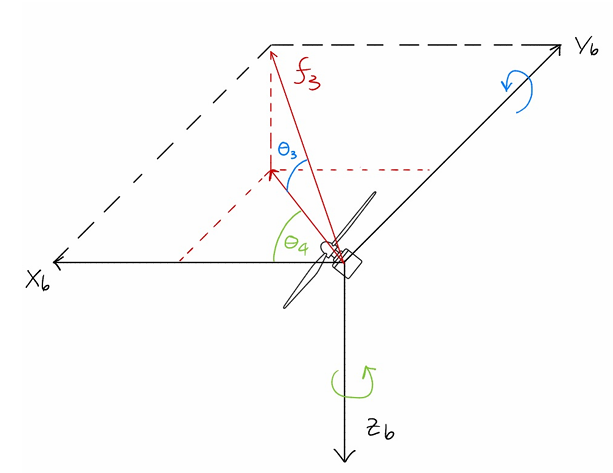
\includegraphics[width=0.8\linewidth]{rotore_3.png} 
            \vspace{0.1cm}
            \captionof{figure}{\footnotesize Compensazione Torque}
        \end{column}
    \end{columns}
\end{frame}

% --- SLIDE 2: PANORAMICA (AGGIORNATA A FULL SMC) ---
\begin{frame}{Architettura Gerarchica: Full Cascaded SMC}
    Si adotta un controllo a cascata per disaccoppiare la dinamica traslazione da quella rotazionale:

    \begin{itemize}
        \item \textbf{Outer Loop (Posizione):} \textcolor{blue}{\textbf{Sliding Mode Control (SMC)}}.
        \begin{itemize}
            \item Tracking di traiettoria e reiezione disturbi atmosferici.
            \item Genera l'assetto desiderato ($\phi_{des}, \theta_{des}$).
        \end{itemize}
        
        \vspace{0.3cm}
        \item \textbf{Inner Loop (Assetto):} \textcolor{red}{\textbf{Sliding Mode Control (SMC)}}.
        \begin{itemize}
            \item \textbf{Robustezza:} Invarianza rispetto alle incertezze della matrice d'inerzia $J$.
            \item \textbf{Velocità:} Tracking istantaneo dei riferimenti angolari esterni.
            \item \textbf{Disaccoppiamento:} Gestione intrinseca dei termini giroscopici non lineari.
        \end{itemize}
    \end{itemize}
    
    \vspace{0.5cm}
    \begin{block}{Vantaggio dell'Architettura Full SMC}
        L'intera catena di controllo condivide la stessa filosofia di stabilità (Lyapunov), garantendo prestazioni superiori rispetto al PID classico in presenza di forti non-linearità.
    \end{block}
\end{frame}

% --- SLIDE 3: SCHEMA A BLOCCHI (Il tuo TikZ originale) ---
\begin{frame}{Schema a Blocchi: Hovering}
    \begin{figure}
        \centering
        \resizebox{0.68\textwidth}{!}{
            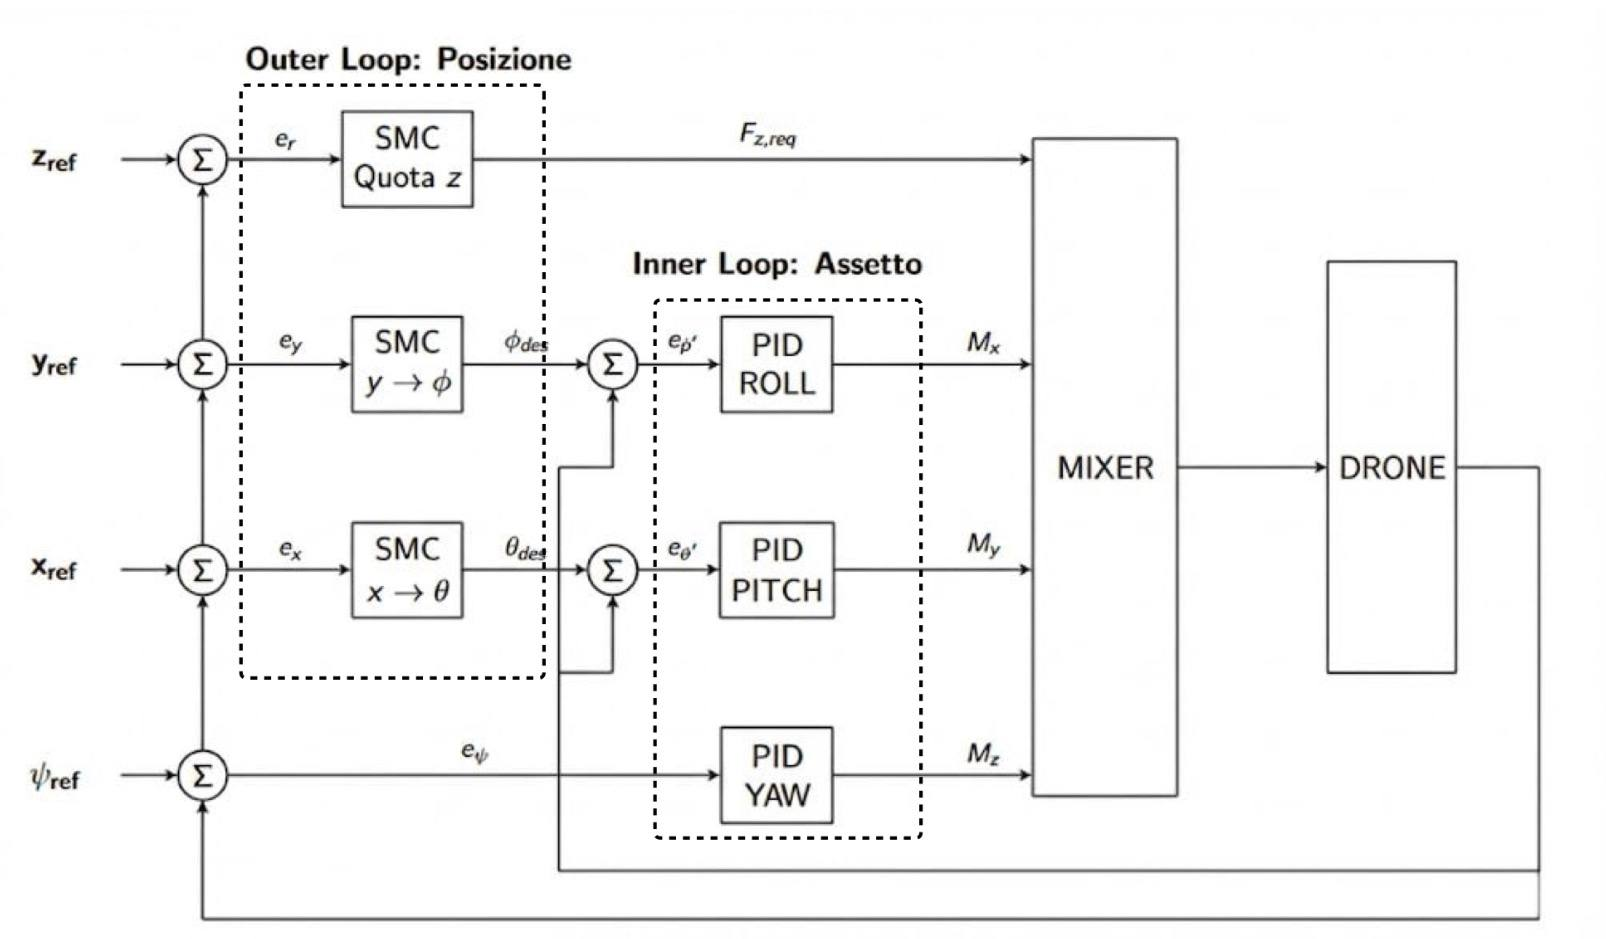
\includegraphics{controllo_verticale/schema_blocchi_V.png}
        }
        \caption{Schema a blocchi del controllo verticale.}
    \end{figure}
\end{frame}

% --- SLIDE 4: SMC QUOTA (INVARIATA) ---
\begin{frame}{Outer Loop: Controllo di Quota}
    \begin{columns}[T]
        \begin{column}{0.6\textwidth}
            \textbf{Obiettivo:} Robustezza ai disturbi.\\
            \vspace{0.2cm}
            \textbf{1. Definizioni:}
            \begin{itemize}
                \item Errore: $e_z = z_{des} - z$
                \item Sliding surface: $\sigma_z = \dot{e}_z + \lambda_z e_z$
            \end{itemize}
            \vspace{0.3cm}
            \textbf{2. Legge di Controllo ($F_{z,req}$):}
            \begin{equation*}
                 \underbrace{mg + F_{aero,z} - m \lambda_z \dot{e}_z}_{\text{Termine Equivalente}} - \underbrace{m K_z \tanh\left(\frac{\sigma_z}{\Phi}\right)}_{\text{Termine Robusto}}
            \end{equation*}
            \small
            L'uso di $\tanh(\cdot)$ al posto di $\text{sgn}(\cdot)$ definisce un \textit{boundary layer} $\Phi$ per eliminare il \textit{chattering}.
        \end{column}
        \begin{column}{0.4\textwidth}
            \centering
            \vspace{0.5cm}
            \begin{tikzpicture}[scale=0.8, >=latex]
                \draw[->] (-2,0) -- (2,0) node[right] {$\sigma$};
                \draw[->] (0,-1.5) -- (0,1.5) node[above] {$u_{rob}$};
                \draw[red, dashed, thick] (-1.8,-1) -- (0,-1) -- (0,1) -- (1.8,1);
                \node[red, font=\scriptsize] at (1.5, 1.2) {sgn};
                \draw[blue, thick, domain=-1.8:1.8, samples=50] plot (\x, {tanh(2*\x)});
                \node[blue, font=\scriptsize] at (1.5, 0.6) {tanh};
                \draw[<->, gray] (-0.5, -0.2) -- (0.5, -0.2);
                \node[gray, below, font=\tiny] at (0, -0.2) {$\Phi$};
            \end{tikzpicture}
            \captionof{figure}{\footnotesize Smoothing dell'azione di controllo.}
        \end{column}
    \end{columns}
\end{frame}

% --- SLIDE 5: STABILITÀ (INVARIATA) ---
\begin{frame}{Analisi di Stabilità}
    Per garantire la stabilità asintotica globale della \textit{sliding surface} ($\sigma \to 0$), si utilizza il criterio di Lyapunov.
    \vspace{0.3cm}
    \begin{columns}[T]
        \begin{column}{0.6\textwidth}
            \textbf{1. Funzione Candidata:}
            \begin{equation*}
                V(\sigma) = \frac{1}{2}\sigma^2 > 0
            \end{equation*}
            \textbf{2. Derivata Temporale:}
            Sostituendo la dinamica a ciclo chiuso con disturbo $\Delta$:
            \begin{align*}
                \dot{V} &= \sigma \dot{\sigma} \\
                        &= -k \sigma \text{sgn}(\sigma) + \sigma \Delta \\
                        &\le -k |\sigma| + |\sigma| \delta_{\max}
            \end{align*}
        \end{column}
        \begin{column}{0.4\textwidth}
            \centering
            \vspace{1cm}
            \begin{alertblock}{Condizione di Stabilità}
                Affinché la funzione decresca ($\dot{V} < 0$), il guadagno deve essere maggiore del disturbo:
                \vspace{0.2cm}
                \centering
                \large
                \boldmath
                $k > \delta_{\max}$
                \unboldmath
            \end{alertblock}
            \small \itshape
            Il sistema è robusto se il guadagno di switching supera il limite superiore dell'incertezza.
        \end{column}
    \end{columns}
\end{frame}

% --- SLIDE 6: GUADAGNI E DISTURBI (INVARIATA) ---
\begin{frame}{Gestione dei Disturbi e Tuning del Guadagno}
    Il vantaggio principale dello SMC è che non richiede la conoscenza puntuale del disturbo $d(t)$, ma solo del suo upper bound.
    \begin{columns}[c]
        \begin{column}{0.5\textwidth}
            \textbf{Condizione di Robustezza:}
            $$ k > |\Delta(t)|_{\max} $$
            \small
            \begin{itemize}
                \item \textcolor{green!60!black}{\textbf{Guadagno Ottimale:}} $k$ leggermente superiore al disturbo massimo atteso. Stabilità garantita e chattering ridotto.
                \item \textcolor{red}{\textbf{Guadagno Eccessivo:}} Stabilità garantita, ma forte chattering e stress sugli attuatori.
                \item \textcolor{orange}{\textbf{Guadagno Insufficiente:}} Perdita di stabilità.
            \end{itemize}
        \end{column}
        \begin{column}{0.5\textwidth}
            \centering
            \begin{tikzpicture}[scale=0.8]
                \draw[->] (0,0) -- (5,0) node[right] {$t$};
                \draw[->] (0,-2.5) -- (0,2.5) node[above] {Ampiezza};
                \draw[gray, thick, domain=0:4.5, samples=100] plot (\x, {1.2*sin(deg(\x*3)) + 0.5*sin(deg(\x*10))});
                \node[gray, right] at (4.5, -0.5) {$d(t)$};
                \draw[dashed, red] (0, 1.8) -- (4.5, 1.8);
                \draw[dashed, red] (0, -1.8) -- (4.5, -1.8);
                \node[red, font=\tiny] at (0.5, 1.9) {$\delta_{max}$};
                \draw[blue, thick] (0, 2.0) -- (4.5, 2.0) node[right] {$k_{buono}$};
                \draw[blue, thick] (0, -2.0) -- (4.5, -2.0);
                \fill[blue, opacity=0.1] (0,-2) rectangle (4.5,2);
            \end{tikzpicture}
            \captionof{figure}{\footnotesize Il guadagno $k$ (blu) deve contenere il disturbo (grigio).}
        \end{column}
    \end{columns}
\end{frame}

% --- SLIDE 7: INVERSIONE CINEMATICA (IL PONTE) ---
\begin{frame}{Inversione Cinematica: Dal Loop Esterno all'Interno}
    Le forze virtuali generate dagli SMC di posizione ($F_{x,req}, F_{y,req}$) devono essere tradotte in angoli di assetto, sfruttando la natura sottoattuata del drone.
    
    \vspace{0.4cm}
    \begin{columns}[c]
        \begin{column}{0.48\textwidth}
            \begin{block}{Generazione Rollio ($\phi_{des}$)}
                \begin{equation}
                    \phi_{des} = \arcsin\left( \frac{F_{y,req}}{T} \right)
                \end{equation}
            \end{block}
        \end{column}
        
        \hfill 
        
        \begin{column}{0.48\textwidth}
            \begin{block}{Generazione Beccheggio ($\theta_{des}$)}
                \begin{equation}
                    \theta_{des} = \arcsin\left( - \frac{F_{x,req}}{T} \right)
                \end{equation}
            \end{block}
        \end{column}
    \end{columns}
    
    \vspace{0.4cm}
    \begin{itemize}
        \item \textbf{Input:} Forze $F_{req}$ robuste (SMC esterno).
        \item \textbf{Output:} Riferimenti angolari $\mathbf{A}_{des}$ per l'SMC interno.
    \end{itemize}
\end{frame}

% --- SLIDE 8: INNER LOOP SMC (IL MOTORE DELLA STABILITÀ) ---
% --- SLIDE 8: INNER LOOP (SMC) ---
\begin{frame}{Inner Loop: Stabilizzazione d'Assetto}
    L'obiettivo è forzare l'errore d'assetto sulla \textbf{sliding surface}, dove il disturbo viene annullato dalla commutazione del controllo.
    \begin{itemize}
    \item Definiamo una condizione di equilibrio dinamico verso cui l'errore deve tendere:
    \begin{equation*}
        \sigma = \dot{e} + \lambda e \quad \longrightarrow \quad \text{se } \sigma=0, \text{ l'errore decade esponenzialmente.}
    \end{equation*}

    \item Il momento richiesto ai motori si compone di due termini:
    \begin{equation*}
        M_{req} = \underbrace{J \lambda \dot{e}}_{\text{Inseguimento Nominale}} + \underbrace{K \tanh(s / \Phi)}_{\text{Reiezione Disturbi}}
    \end{equation*}
    \end{itemize}

    Vengono generati dei momenti torcenti lungo gli assi $x, y, z$ attraverso i quali si raggiungono gli angoli desiderati.
\end{frame}

% --- SLIDE 8: MMA Longitudinale (Condensata) ---
\begin{frame}{Motor Mixing Algorithm: Longitudinale}
    La dinamica longitudinale richiede la risoluzione di un sistema accoppiato: Spinta ($T$) e Beccheggio ($M_y$).
    
    \vspace{0.3cm}
    \textbf{1. Calcolo Rotore di Coda ($\omega_3$):}
    Dall'equilibrio dei momenti attorno a Y, si isola il contributo della coda:
    \begin{equation}
        \omega_3 = \sqrt{\frac{M_{y,req} - F_{z,req} d_{mx}}{k \sin(\theta_3) (d_{tx} - d_{mx}) + b \cos(\theta_3) \sin(\theta_4)}}
    \end{equation}
    
    \vspace{0.3cm}
    \textbf{2. Calcolo Rotori Anteriori ($T_{front}$):}
    Nota la spinta della coda, il resto del sostentamento è affidato ai rotori anteriori:
    \begin{equation}
        T_{front} = F_{z,req} - T_3 \sin(\theta_3)
    \end{equation}
\end{frame}

% --- SLIDE 9: MMA Laterale (Condensata) ---
\begin{frame}{Motor Mixing Algorithm: Latero-Direzionale}
    Una volta determinato $T_{front}$, questo viene modulato per controllare Roll e Yaw.
    
    \vspace{0.5cm}
    \begin{columns}[T]
        \begin{column}{0.48\textwidth}
            \textbf{ROLL (Spinta Differenziale)} \\
            Si ripartisce la spinta anteriore tra destra ($T_1$) e sinistra ($T_2$):
            \begin{equation}
                \Delta\omega_{des} = \frac{M_{x,req}}{2 d_{my}}
            \end{equation}
            \begin{equation}
                \begin{cases}
                    \omega_{1} = \frac{T_{front}}{2k} - \Delta\omega_{des}\\
                    \omega_{2} = \frac{T_{front}}{2k} + \Delta\omega_{des}
                \end{cases}
            \end{equation}
        \end{column}
        \begin{column}{0.48\textwidth}
            \textbf{YAW (Tilt Differenziale)} \\
            Si inclina il vettore spinta anteriore per creare coppia su Z:
            \begin{equation}
                \delta_{des} = \arcsin\left( \frac{M_{z,req}}{T_{front} d_{my}} \right)
            \end{equation}
            \begin{equation}
                \begin{cases}
                    \theta_1 = \pi/2 - \delta_{des}\\
                    \theta_2 = \pi/2 + \delta_{des}
                \end{cases}
            \end{equation}
            
        \end{column}
    \end{columns}
\end{frame}

% % ===========================================================
% % SIMULAZIONI (RIELABORATE)
% % ==========================================================
% \section{Simulazioni controllo verticale}

% \begin{frame}
%     \vfill
%     \centering
%     {\Huge \textbf{Risultati Simulazione}}
%     \vfill
% \end{frame}

% % --- SLIDE SIMULAZIONI 1: Assetto ---
% \begin{frame}{Analisi Prestazionale: Assetto}
%     \begin{columns}[c]
%         \begin{column}{0.65\textwidth}
%             \centering
%             
\includegraphics[width=\linewidth]{angoli.png}
%         \end{column}
%         \begin{column}{0.35\textwidth}
%             \textbf{Risposta Angolare:}
%             \begin{itemize}
%                 \item \textcolor{blue!80!black}{\textbf{Velocità:}} Settling time < 2s.
%                 \item \textcolor{blue!80!black}{\textbf{Precisione:}} Errore a regime nullo sugli angoli di Eulero.
%                 \item \textcolor{blue!80!black}{\textbf{Overshoot:}} Minimo (< 5\%) durante i transitori.
%             \end{itemize}
%         \end{column}
%     \end{columns}
% \end{frame}

% \begin{frame}{Analisi Prestazionale: Posizione}
%     \begin{columns}[c]
%         \begin{column}{0.65\textwidth}
%             \centering
%             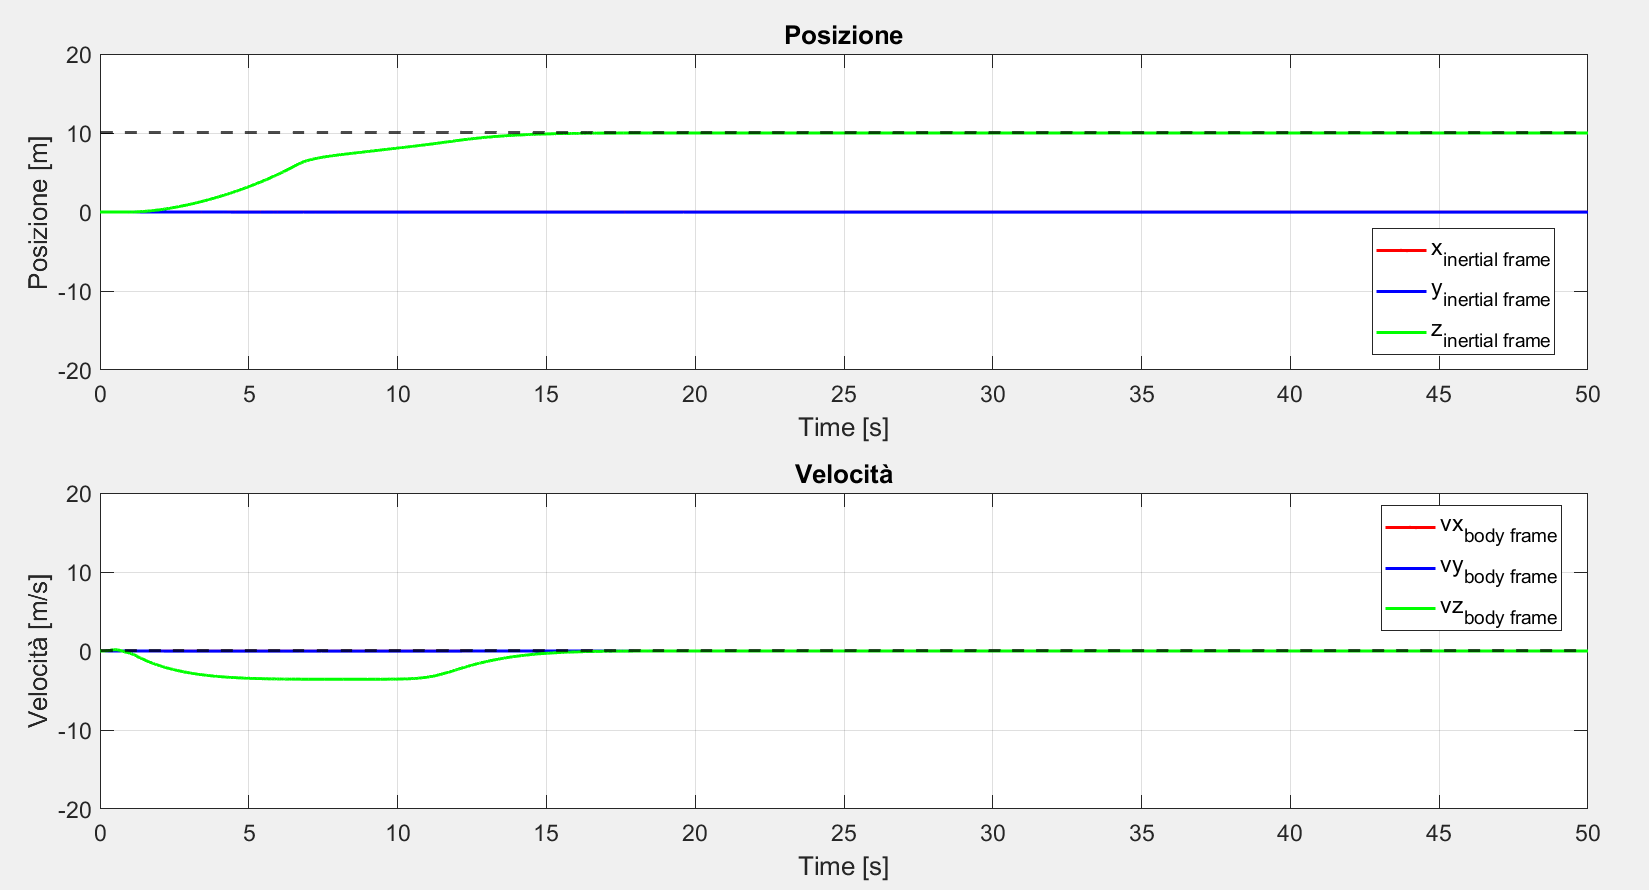
\includegraphics[width=\linewidth]{pos_vel.png}
%         \end{column}
%         \begin{column}{0.35\textwidth}
%             \textbf{Posizione inerziale:}
%             \begin{itemize}
%                 \item \textcolor{blue!80!black}{\textbf{X e Y:}} Il drone rimane fermo lungo gli assi $x$ e $y$.
%                 \item \textcolor{blue!80!black}{\textbf{Z:}} Viene raggiunta con successo la quota.
%             \end{itemize}
%         \end{column}
%     \end{columns}
% \end{frame}

% % --- SLIDE SIMULAZIONI 2: Attuatori ---
% \begin{frame}{Analisi degli Attuatori: Sforzo di Controllo}
%     \begin{columns}[c]
%         \begin{column}{0.65\textwidth}
%             
\includegraphics[width=\linewidth]{thrust.png}
%         \end{column}
%         \begin{column}{0.35\textwidth}
%             \textbf{Thrust:}
%             \begin{itemize}
%                 \item Nessuna saturazione dei motori (Max 100N).
%             \end{itemize}
%         \end{column}
%     \end{columns}
% \end{frame}

% % --- SLIDE SIMULAZIONI 2: Attuatori ---
% \begin{frame}{Analisi degli Attuatori: Sforzo di Controllo}
%     \begin{columns}[c]
%         \begin{column}{0.65\textwidth}
%             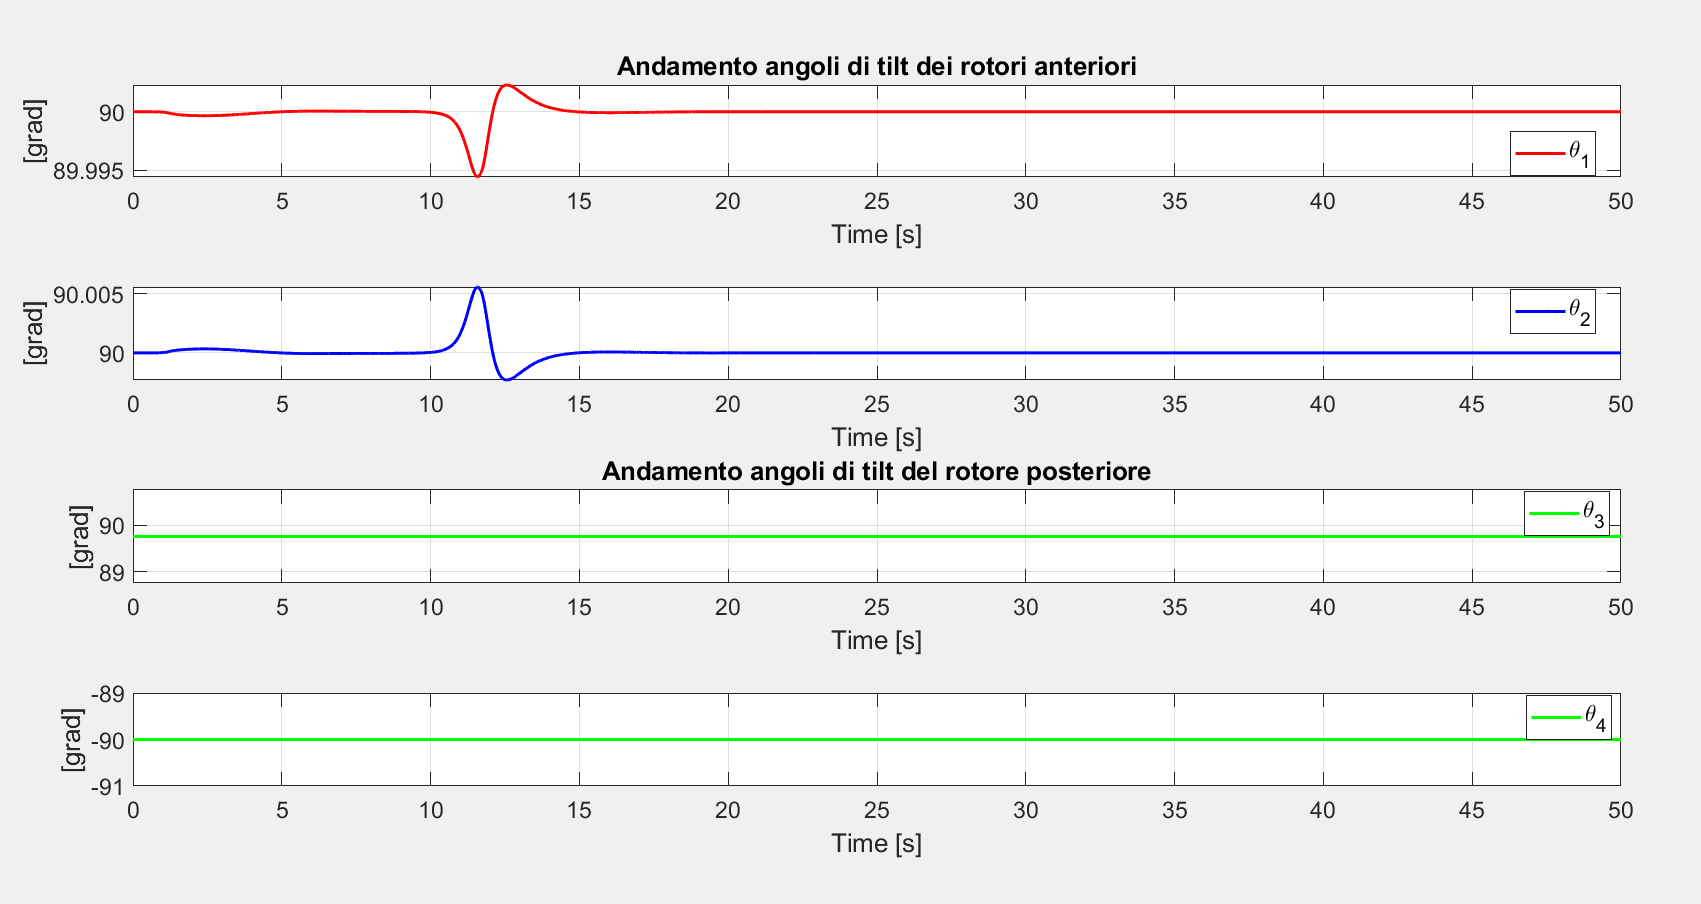
\includegraphics[width=\linewidth]{tilt.png}
%         \end{column}
%         \begin{column}{0.35\textwidth}
%             \textbf{Tilt:}
%             \begin{itemize}
%                 \item Escursione contenuta ($\pm 5^\circ$) in hovering.
%                 \item Dinamica compatibile con la banda passante dei servi.
%             \end{itemize}
%         \end{column}
%     \end{columns}
% \end{frame}


% ============================================================
% 4. CONTROLLO ORIZZONTALE (RIELABORATO)
% ============================================================
\section{Controllo Volo Orizzontale}

\begin{frame}
    \vfill
    \centering
    {\Huge \textbf{Controllo Orizzontale}}
    \vfill
\end{frame}

% --- SLIDE 1: CONFIGURAZIONE CROCIERA ---
\begin{frame}{Configurazione di Crociera (Fixed-Wing Mode)}
    Durante il volo avanzato, i rotori anteriori generano spinta propulsiva orizzontale.
    
    \vspace{0.3cm}
    \begin{columns}[c]
        \begin{column}{0.6\textwidth}
            \textbf{Configurazione:}
            \begin{itemize}
                \item Rotori Anteriori: $\theta \approx 0^\circ$ (Orizzontali).
                \item Rotore di Coda: \textbf{Spento} (per evitare instabilità intorno all'asse X).
            \end{itemize}
            
            \vspace{0.3cm}
            \begin{alertblock}{La Sfida di Controllo}
                Il velivolo è \textbf{sotto-attuato} e privo di superfici aerodinamiche mobili (alettoni, flap, timone).
                Tutto il controllo di assetto è affidato al \textbf{Thrust Vectoring} dei soli due rotori anteriori.
            \end{alertblock}
        \end{column}
        
        \begin{column}{0.4\textwidth}
            \centering
            % Placeholder per immagine drone in volo orizzontale
            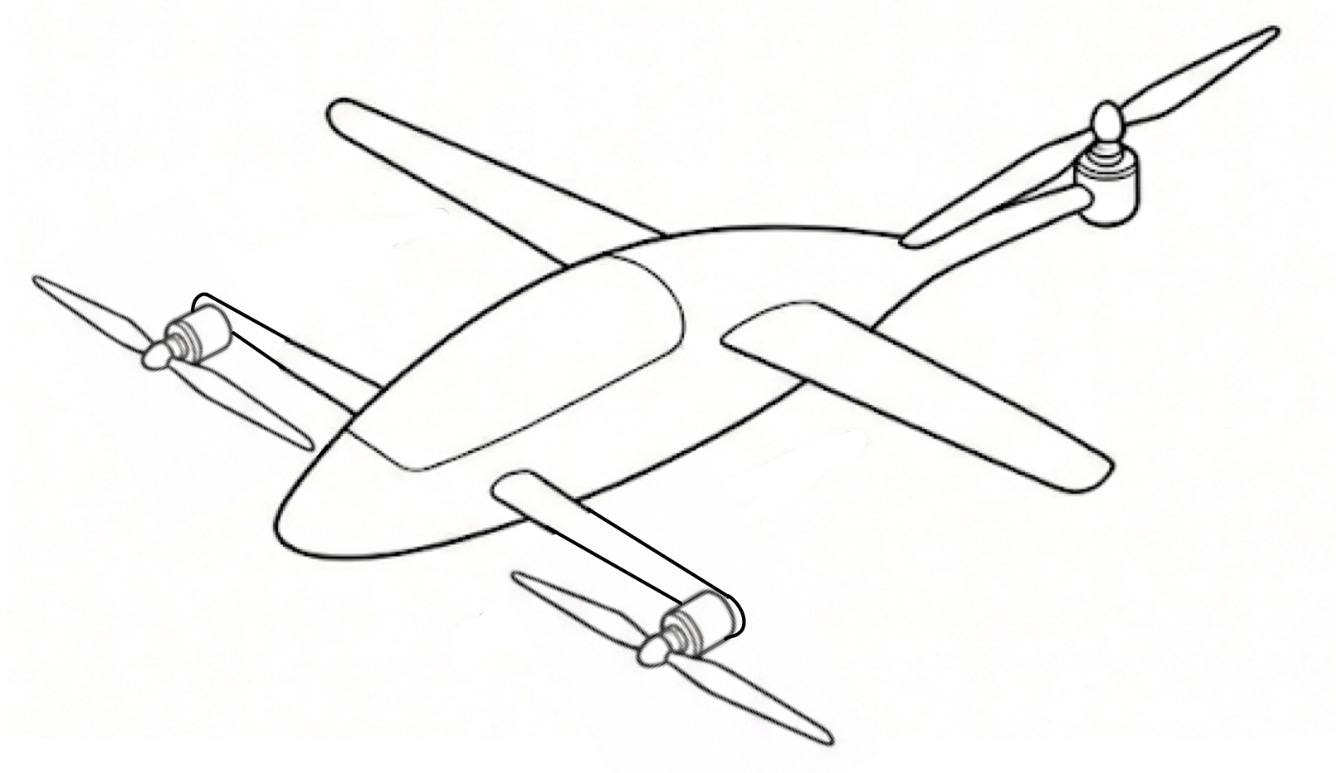
\includegraphics[width=0.9\linewidth]{config_orizzontale.png} 
            \captionof{figure}{\footnotesize Configurazione Forward Flight}
        \end{column}
    \end{columns}
\end{frame}

\begin{frame}{Architettura Gerarchica: PID}
    Si adotta un controllo a cascata per disaccoppiare la dinamica traslazione da quella rotazionale:

    \begin{itemize}
        \item \textbf{Outer Loop (Posizione e Velocità):} \textcolor{blue}{\textbf{PID}}.
        \begin{itemize}
            \item Mantenimento della quota e raggiungimento della velocità di crociera.
        \end{itemize}
        
        \vspace{0.3cm}
        \item \textbf{Inner Loop (Assetto):} \textcolor{red}{\textbf{PID}}.
        \begin{itemize}
            \item Richiesta di asservimento degli angoli di assetto nulli.
        \end{itemize}
    \end{itemize}
    
    \vspace{0.5cm}
    \begin{block}{Vantaggio dell'Architettura PID}
        A velocità elevate ($25 \text{ m/s}$), le forze aerodinamiche stabilizzano naturalmente il velivolo. Il PID, con termini di \textbf{Feedforward}, garantisce efficienza energetica, fluidità e minor stress meccanico rispetto allo SMC.
    \end{block}
\end{frame}

\begin{frame}{Schema a Blocchi: Crociera}
    \begin{figure}
        \centering
        \resizebox{0.75\textwidth}{!}{
            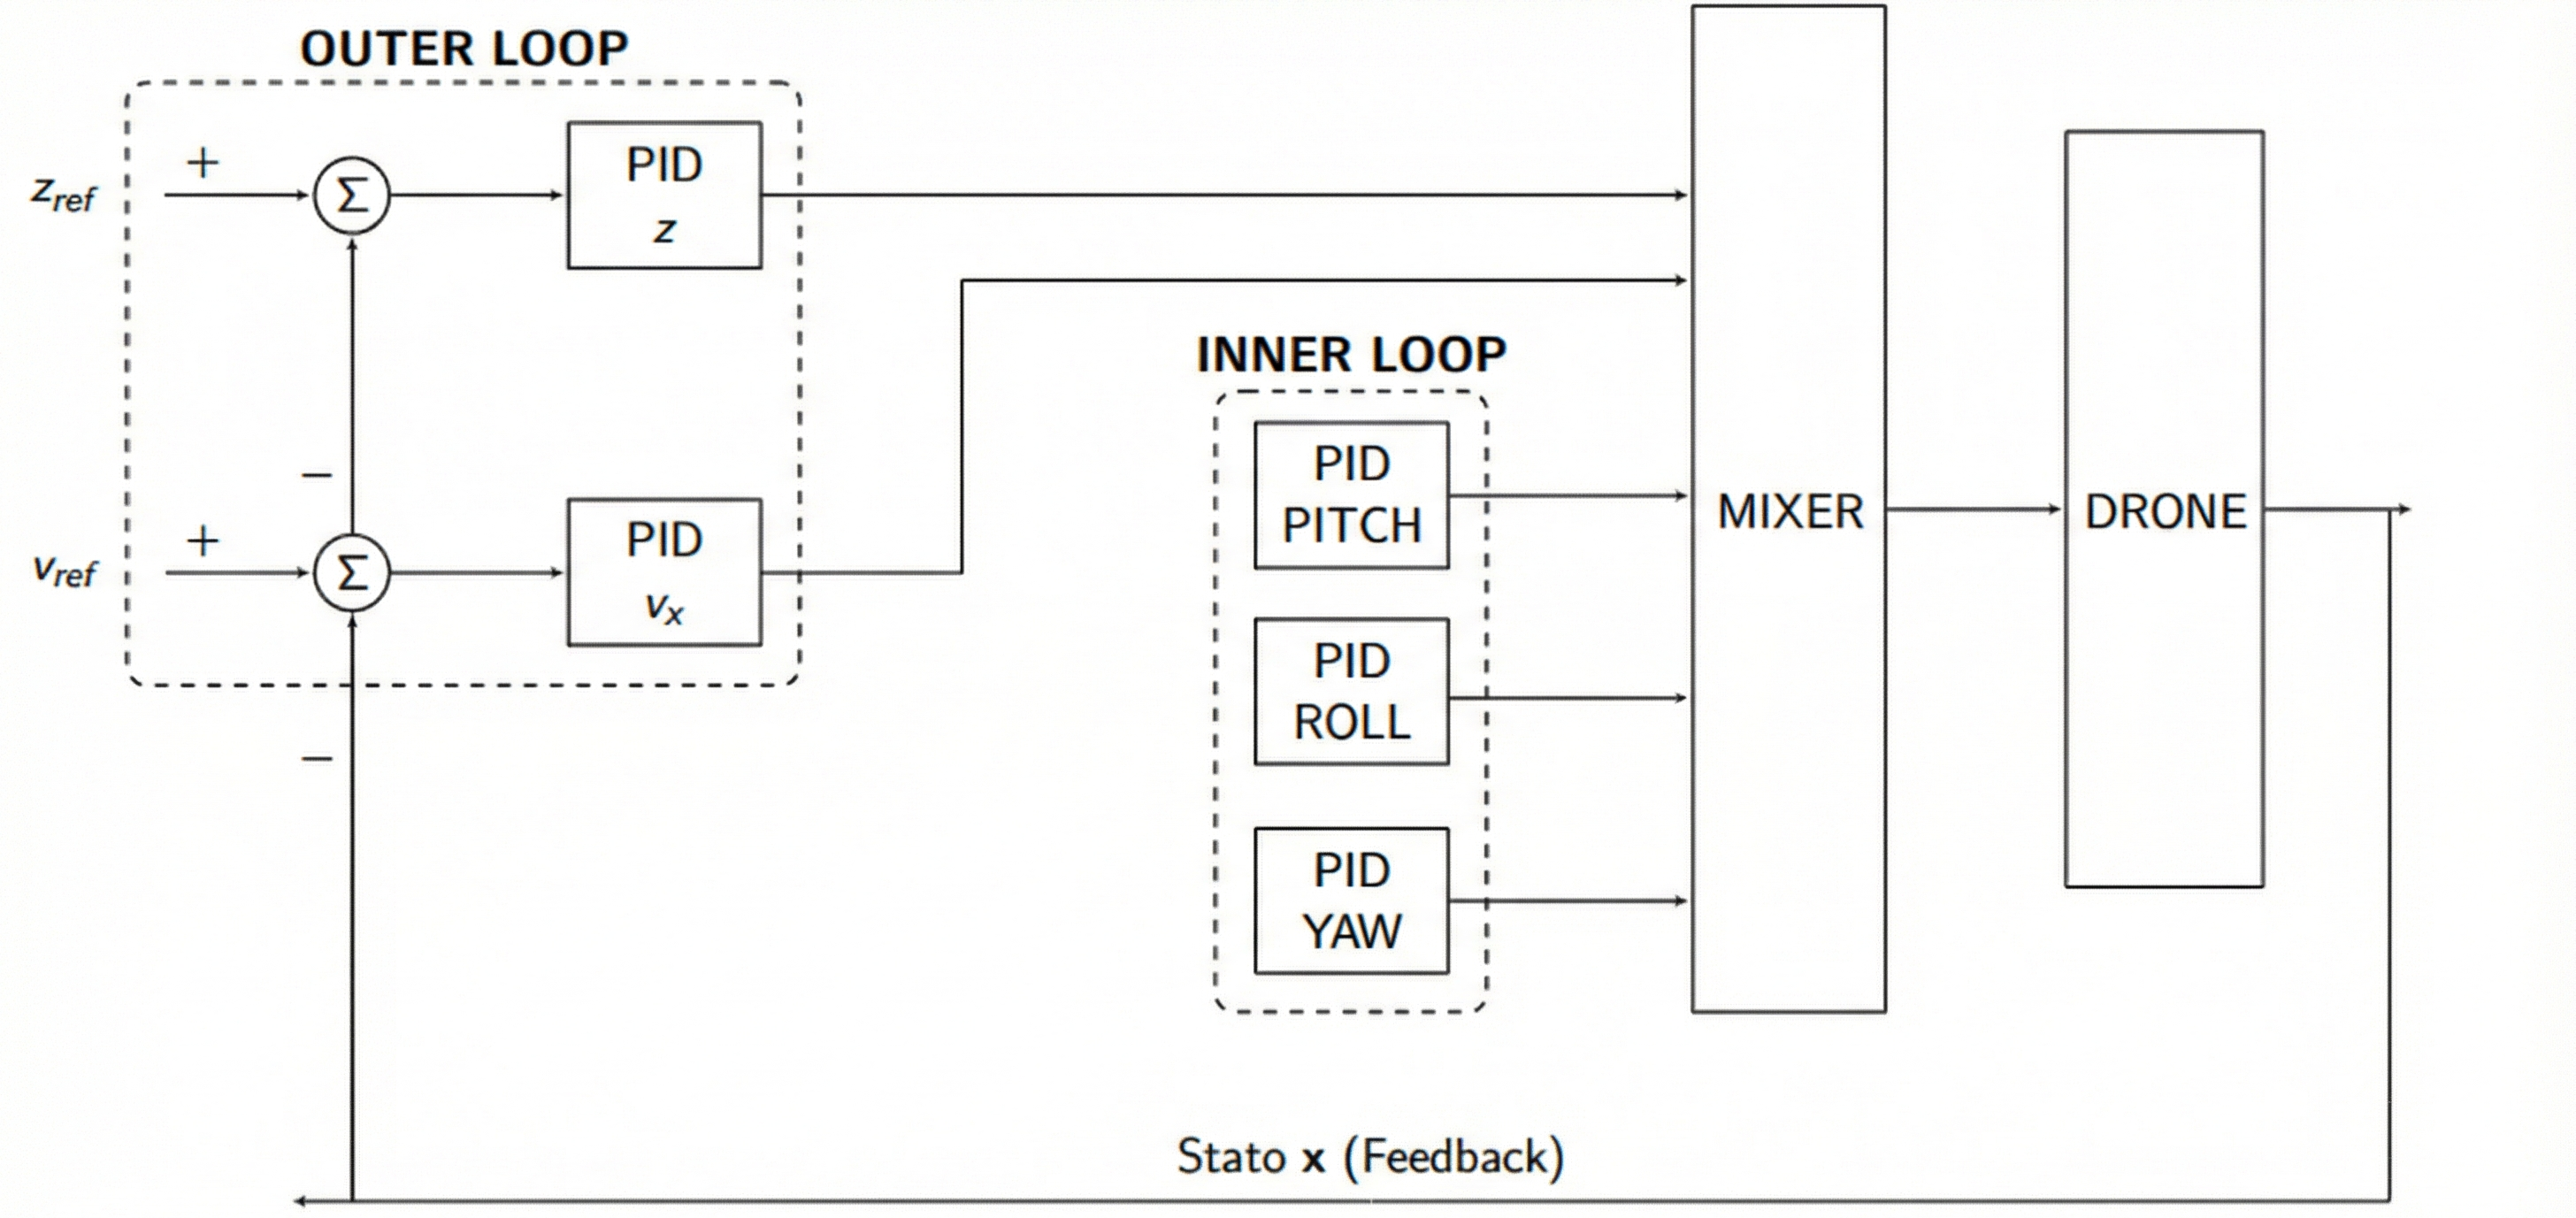
\includegraphics{controllo_orizzontale/schema_blocchi_H.png}
        }
        \caption{Schema a blocchi del controllo orizzontale.}
    \end{figure}
\end{frame}



% % --- SLIDE 2: SCHEMA A BLOCCHI (Il tuo TikZ) ---
% \begin{frame}{Schema a blocchi: Controllo Orizzontale}
%     \begin{figure}[htbp]
%     \centering
%     \resizebox{0.8\textwidth}{!}{
%     \begin{tikzpicture}[auto, node distance=1.3cm, >=Stealth, thick]
%         % --- STILI ---
%         \tikzset{
%             block/.style={draw, rectangle, minimum height=3em, minimum width=4.5em, align=center, fill=white},
%             sum/.style={draw, circle, inner sep=0pt, minimum size=6mm},
%             input/.style={coordinate},
%             output/.style={coordinate},
%             container/.style={draw, rectangle, rounded corners, dashed, inner sep=0.4cm}
%         }

%         % --- COLONNA 1: OUTER LOOP ---
%         \node [input] (ref_z) {};
%         \node [sum, right=0.8cm of ref_z] (sum_z) {$\Sigma$};
%         \node [block, right=1cm of sum_z] (pid_z) {PID\\$z$};
%         \node [left=0.1cm of ref_z] {$z_{des}$};

%         \node [input, below=1.5cm of ref_z] (ref_vx) {};
%         \node [sum, right=0.8cm of ref_vx] (sum_vx) {$\Sigma$};
%         \node [block, right=1cm of sum_vx] (pid_vx) {PID\\$v_x$};
%         \node [left=0.1cm of ref_vx] {$v_{x,des}$};

%         % \node [input, below=3.5cm of ref_vx] (ref_y) {};
%         % \node [sum, right=0.8cm of ref_y] (sum_y) {$\Sigma$};
%         % \node [block, right=1cm of sum_y] (pid_y) {PID\\$y$};
%         % \node [left=0.1cm of ref_y] {$y_{des}$};

%         % --- COLONNA 2: INNER LOOP ---
%         \node [sum, right=3cm of pid_vx, yshift=-1.5cm] (sum_theta) {$\Sigma$};
%         \node [block, right=0.8cm of sum_theta] (pid_theta) {PID\\$\theta$};
        
%         \node [sum, below=1cm of sum_theta] (sum_phi) {$\Sigma$};
%         \node [block, right=0.8cm of sum_phi] (pid_phi) {PID\\$\phi$};

%         \node [sum, below=1cm of sum_phi] (sum_psi) {$\Sigma$};
%         \node [block, right=0.8cm of sum_psi] (pid_psi) {PID\\$\psi$};

%         % --- COLONNA 3: MIXER E DRONE ---
%         \node [block, right=8.5cm of pid_vx, minimum height=10.5cm, yshift=-2cm] (mixer) {MMA};
%         \node [block, right=1.5cm of mixer, minimum height=8.5cm] (drone) {DRONE};
%         \node [output, right=1cm of drone] (drone_out) {};

%         % --- CONNESSIONI DIRETTE ---
%         \draw [->] ($(sum_theta.west)-(0.8,0)$) -- node[above, pos=0] {$\theta_{des}$} (sum_theta.west);
%         \draw [->] ($(sum_phi.west)-(0.8,0)$) -- node[above, pos=0] {$\phi_{des}$} (sum_phi.west);
%         \draw [->] ($(sum_psi.west)-(0.8,0)$) -- node[above, pos=0] {$\psi_{des}$} (sum_psi.west);

%         \draw [->] (pid_z.east) -- (mixer.west |- pid_z.east) node[above, pos=0.15] {$F_{z,req}$};
%         \draw [->] (pid_vx.east) -- (mixer.west |- pid_vx.east) node[above, pos=0.15] {$F_{x,req}$};
%         \draw [->] (pid_theta.east) -- (mixer.west |- pid_theta.east) node[above, pos=0.5] {$\theta_{pitch}$};
%         \draw [->] (pid_phi.east) -- (mixer.west |- pid_phi.east) node[above, pos=0.5] {$\delta$};
%         \draw [->] (pid_psi.east) -- (mixer.west |- pid_psi.east) node[above, pos=0.5] {$\Delta \omega$};

%         \draw [->] (ref_z) -- (sum_z); \draw [->] (sum_z) -- (pid_z);
%         \draw [->] (ref_vx) -- (sum_vx); \draw [->] (sum_vx) -- (pid_vx);
%         % \draw [->] (ref_y) -- (sum_y); \draw [->] (sum_y) -- (pid_y);
%         % \draw [->] (pid_y.east) -- node[above] {$\phi_{des}$} (sum_phi.west);
%         \draw [->] (sum_theta) -- (pid_theta);
%         \draw [->] (sum_phi) -- (pid_phi);
%         \draw [->] (sum_psi) -- (pid_psi);
%         \draw [->] (mixer) -- (drone);
%         \draw [->] (drone) -- (drone_out);

%         % --- FEEDBACK BUS ---
%         \coordinate (fb_node) at ($(drone.east)+(0.5,0)$);
%         \coordinate (line_outer) at (0,-9.8); % Bus per Outer Loop
%         \coordinate (line_inner) at (0,-9);    % Bus per Inner Loop

%         \draw (fb_node) |- (line_outer) -- ($(sum_z.west |- line_outer)$);
%         \draw (fb_node) |- (line_inner) -- ($(sum_theta.west |- line_inner)$);

%         \draw [->, shorten >=0.5pt] (sum_z.south |- line_outer) -- (sum_z.south) node[left, pos=0.85] {$-$};
%         \draw [->, shorten >=0.5pt] (sum_vx.south |- line_outer) -- (sum_vx.south) node[left, pos=0.85] {$-$};
%         % \draw [->, shorten >=0.5pt] (sum_y.south |- line_outer) -- (sum_y.south) node[left, pos=0.85] {$-$};

%         \draw [->, shorten >=0.5pt] (sum_theta.south |- line_inner) -- (sum_theta.south) node[left, pos=0.7] {$-$};
%         \draw [->, shorten >=0.5pt] (sum_phi.south |- line_inner) -- (sum_phi.south) node[left, pos=0.7] {$-$};
%         \draw [->, shorten >=0.5pt] (sum_psi.south |- line_inner) -- (sum_psi.south) node[left, pos=0.85] {$-$};

%         % --- CONTAINERS ---
%         \begin{scope}[on background layer]
%             \node [container, draw, fit=(sum_z) (pid_z) (sum_vx) (pid_vx), label={above:\textbf{Outer Loop}}] {};
%             \node [container, draw, fit=(sum_theta) (pid_theta) (sum_psi) (pid_psi), label={below:\textbf{Inner Loop}}] {};
%         \end{scope}

%     \end{tikzpicture}
%     }
%     \caption{Architettura a Cascata: Guidance (Lento) e Attitude (Veloce).}
%     \end{figure}
% \end{frame}

% --- SLIDE 3: OUTER LOOP (UNIFICATA) ---
\begin{frame}{Outer Loop: Quota e Velocità}
    L'Outer Loop genera le forze richieste ($F_{req}$) per inseguire i riferimenti. Entrambi i canali utilizzano un Feedforward Aerodinamico.

    \vspace{0.3cm}
    \begin{columns}[T]
        % Colonna Quota
        \begin{column}{0.48\textwidth}
            \begin{block}{Controllo Quota ($z$)}
                Mantenimento altitudine tramite modulazione forza verticale:
                \begin{equation}
                    F_{z,req} = \underbrace{m (g - a_{z,PID})}_{\text{Inerziale}} - \underbrace{L_{wing}(v)}_{\text{Lift Feedforward}}
                \end{equation}
            \end{block}
        \end{column}

        % Colonna Velocità
        \begin{column}{0.48\textwidth}
            \begin{block}{Controllo Velocità ($v_x$)}
                Inseguimento del setpoint ($25 m/s$) tramite forza propulsiva:
                \begin{equation}
                    F_{x,req} = \underbrace{F_{x,PID}}_{\text{Correttivo}} + \underbrace{D_{x}(v)}_{\text{Drag Feedforward}}
                \end{equation}
            \end{block}
        \end{column}
    \end{columns}

\end{frame}

% \begin{frame}{Outer Loop: Inseguimento Traiettoria (PID vs SMC)}
%     Il loop esterno gestisce la quota ($z$) e la velocità ($v_x$).
%     \vspace{0.2cm}
%     Il passaggio allo Sliding Mode risolve i limiti del controllo lineare.
    
%     \begin{columns}[T]
%         \begin{column}{0.48\textwidth}
%             \begin{block}{Approccio PID + FF}
%                 \centering 
%                 $F_{z,req} = m(g - a_{z,PID}) - L_{wing}$ \\
%                 $F_{x,req} = F_{x,PID} + D_{wing}$
%                 \begin{itemize}
%                     \item Richiede errore residuo per compensare mismatch del modello.
%                     \item Non stressa i motori per fluttuazioni gestibili tramite le ali.
%                 \end{itemize}
%             \end{block}
%         \end{column}
        
%         \begin{column}{0.48\textwidth}
%             \begin{block}{Approccio SMC (Robusto)}
%                 \centering 
%                 $F_{z,req} = (m g - L_{wing}) - m K_z \tanh(s_z/\Phi)$ \\
%                 $F_{x,req} = D_{wing} + K_{v} \tanh(s_v/\Phi)$
%                 \begin{itemize}
%                     \item Interviene non appena lo stato si discosta dalla sliding surface, rivelandosi più robusto.
%                     \item Maggiori consumi e più stress sui motori.
%                 \end{itemize}
%             \end{block}
%         \end{column}
%     \end{columns}
%     \vspace{0.3cm}
%     \textit{Mentre il PID "insegue" l'errore, lo SMC "forza" lo stato sulla superficie desiderata.}
% \end{frame}

% --- SLIDE 4: INNER LOOP (ANALOGIE) ---
\begin{frame}{Inner Loop: Thrust Vectoring come Superfici Virtuali}
    In assenza di alettoni e timoni, il mixer emula le superfici di controllo classiche usando i motori.

    \vspace{0.3cm}
    \begin{columns}[T]
        \begin{column}{0.32\textwidth}
            \begin{alertblock}{Pitch ($\theta$)}
                \centering \textbf{"Elevatori"}
                \vspace{0.2cm}
                \begin{itemize}
                    \item \textbf{Azione:} Tilt Collettivo.
                    \item $\theta_1 = \theta_2$.
                    \item Ruota il vettore spinta su/giù.
                    \item PID
                \end{itemize}
            \end{alertblock}
        \end{column}

        \begin{column}{0.32\textwidth}
            \begin{block}{Roll ($\phi$)}
                \centering \textbf{"Alettoni"}
                \vspace{0.2cm}
                \begin{itemize}
                    \item \textbf{Azione:} Tilt Differenziale.
                    \item $\theta_1 = -\theta_2$.
                    \item Crea coppia torcente sull'asse $X$.
                    \item PD
                \end{itemize}
            \end{block}
        \end{column}

        \begin{column}{0.32\textwidth}
            \begin{exampleblock}{Yaw ($\psi$)}
                \centering \textbf{"Timone"}
                \vspace{0.2cm}
                \begin{itemize}
                    \item \textbf{Azione:} Spinta Differenziale.
                    \item $\omega_1 \neq \omega_2$.
                    \item Crea coppia torcente sull'asse $Z$.
                    \item PD
                \end{itemize}
            \end{exampleblock}
        \end{column}
    \end{columns}
\end{frame}

% % --- SLIDE 5: ANALISI COMPARATIVA ---
% \begin{frame}{Analisi Comparativa: Quando usare cosa?}
%     La scelta tra PID e SMC non è univoca, ma dipende dai requisiti di missione e dall'hardware.

%     \begin{columns}[T]
%         \begin{column}{0.48\textwidth}
%             \begin{exampleblock}{Scegliere il PID se...}
%                 \begin{itemize}
%                     \item \textbf{Hardware limitato:} Richiede bassa potenza computazionale.
%                     \item \textbf{Salute Attuatori:} I segnali sono intrinsecamente morbidi (no vibrazioni).
%                     \item \textbf{Modello Noto:} Il modello fisico è molto preciso.
%                 \end{itemize}
%             \end{exampleblock}
%         \end{column}

%         \begin{column}{0.48\textwidth}
%             \begin{alertblock}{Scegliere lo SMC se...}
%                 \begin{itemize}
%                     \item \textbf{Alta Precisione:} Necessità di tracking millimetrico ($Z, V_x$).
%                     \item \textbf{Robustezza:} Presenza di disturbi (vento) o incertezze (stallo).
%                     \item \textbf{Sottosituazione:} Sistemi complessi come i VTOL Tilt-Rotor.
%                 \end{itemize}
%             \end{alertblock}
%         \end{column}
%     \end{columns}
%     \vspace{0.3cm}
%     \centering
%     \textbf{Conclusione:} Per il prototipo in esame, lo \textbf{SMC} è risultato indispensabile per garantire il 100\% di successo nelle fasi di transizione e crociera.
% \end{frame}

% --- SLIDE 5: MMA CONCETTO (SINTESI VETTORIALE) ---
\begin{frame}{Motor Mixing Algorithm: Sintesi e Compensazione Geometrica}
    Il Mixer traduce le forze cartesiane ($F_x, F_z$) in un vettore spinta.\\
    \vspace{0.3cm}
    \textbf{1. Sintesi del Vettore Spinta (Frame Inerziale)}
    \begin{equation}
        T_{tot} = \sqrt{F_{x}^2 + F_{z}^2} \quad ; \quad \alpha_{inertial} = \arctan2(F_z, F_x)
    \end{equation}

    \vspace{0.3cm}
    \textbf{2. Trasformazione al Body Frame (Compensazione)}
    I servi sono solidali alla fusoliera. Se il drone cabra ($\theta > 0$), i motori devono ruotare in basso per mantenere la spinta orizzontale.
    
    \begin{equation}
        \boxed{\alpha_{base} = \alpha_{inertial} - \theta_{body}}
    \end{equation}
    
    \small \textit{Questo disaccoppia la dinamica di traslazione dalle oscillazioni di beccheggio.}
\end{frame}

% --- SLIDE 6: MMA ATTUAZIONE (EQUAZIONI FINALI) ---
\begin{frame}{Motor Mixing Algorithm: Leggi di Attuazione}
    Ai valori di base si sovrappongono i comandi di stabilizzazione ($u_\phi, u_\psi$) dell'Inner Loop.

    \vspace{0.5cm}
    % L'opzione 'onlytextwidth' assicura che il calcolo delle larghezze sia pulito
    \begin{columns}[c, onlytextwidth] 
        \hfill % Margine sinistro (opzionale, per centrare il blocco totale)
        
        \begin{column}{0.44\textwidth}
            \centering % Centra il contenuto dentro la colonna per staccarlo dai bordi
            \textbf{A. Comandi ai Motori} \\
            (Controllo Yaw e Spinta)
            \begin{equation}
                \begin{cases}
                    \omega_{1} = \frac{T_{tot}}{2k} - u_{\psi} \\
                    \omega_{2} = \frac{T_{tot}}{2k} + u_{\psi}
                \end{cases}
            \end{equation}
            $\implies$ RPM Motori.
        \end{column}
        
        \hfill % Crea lo spazio centrale tra le due colonne
        
        \begin{column}{0.44\textwidth}
            \centering
            \textbf{B. Comandi ai Servi} \\
            (Controllo Pitch e Roll)
            \begin{equation}
                \begin{cases}
                    \theta_{1} = \alpha_{base} + u_{\theta} - u_{\phi} \\
                    \theta_{2} = \alpha_{base} + u_{\theta} + u_{\phi}
                \end{cases}
            \end{equation}
            $\implies$ Angoli Servi.
        \end{column}
        
        \hfill % Margine destro
    \end{columns}
\end{frame}

% ===========================================================
% SEZIONE 5: VALIDAZIONE E ROBUSTEZZA (MONTE CARLO)
% ===========================================================
\section{Validazione Monte Carlo}

\begin{frame}
    \vfill
    \centering
    \Huge \textbf{Validazione Monte Carlo}
    \vfill
\end{frame}

% --- SLIDE 1: METODOLOGIA ---
\begin{frame}{Metodologia di Validazione}
    \begin{alertblock}{Stress-Test stocastico ($N=300$)}
        Il sistema è stato sottoposto a 100 simulazioni per ogni scenario per quantificare la robustezza dei controllori scelti a fronte di incertezze iniziali ($\pm 15^\circ$ assetto, $\pm 2$m posizione) e mismatch dei parametri aerodinamici.
    \end{alertblock}

    \vspace{0.3cm}
            \textbf{Logica di Controllo adottata:}
            \begin{itemize}
                \item \textbf{SMC (Takeoff/Recovery):} Scelto per la gestione delle forti non-linearità e la reiezione dei disturbi in hovering.
                \item \textbf{PID (Cruise):} Utilizzato come baseline per il volo rettilineo uniforme a $25$ m/s.
            \end{itemize}

\end{frame}

% --- SLIDE 2: SMC TAKEOFF ---
\begin{frame}{Scenario 1: Decollo con SMC}
    \textbf{Obiettivo:} Transizione stabile dal suolo alla quota desiderata.
    \vspace{0.2cm}
    \begin{center}
        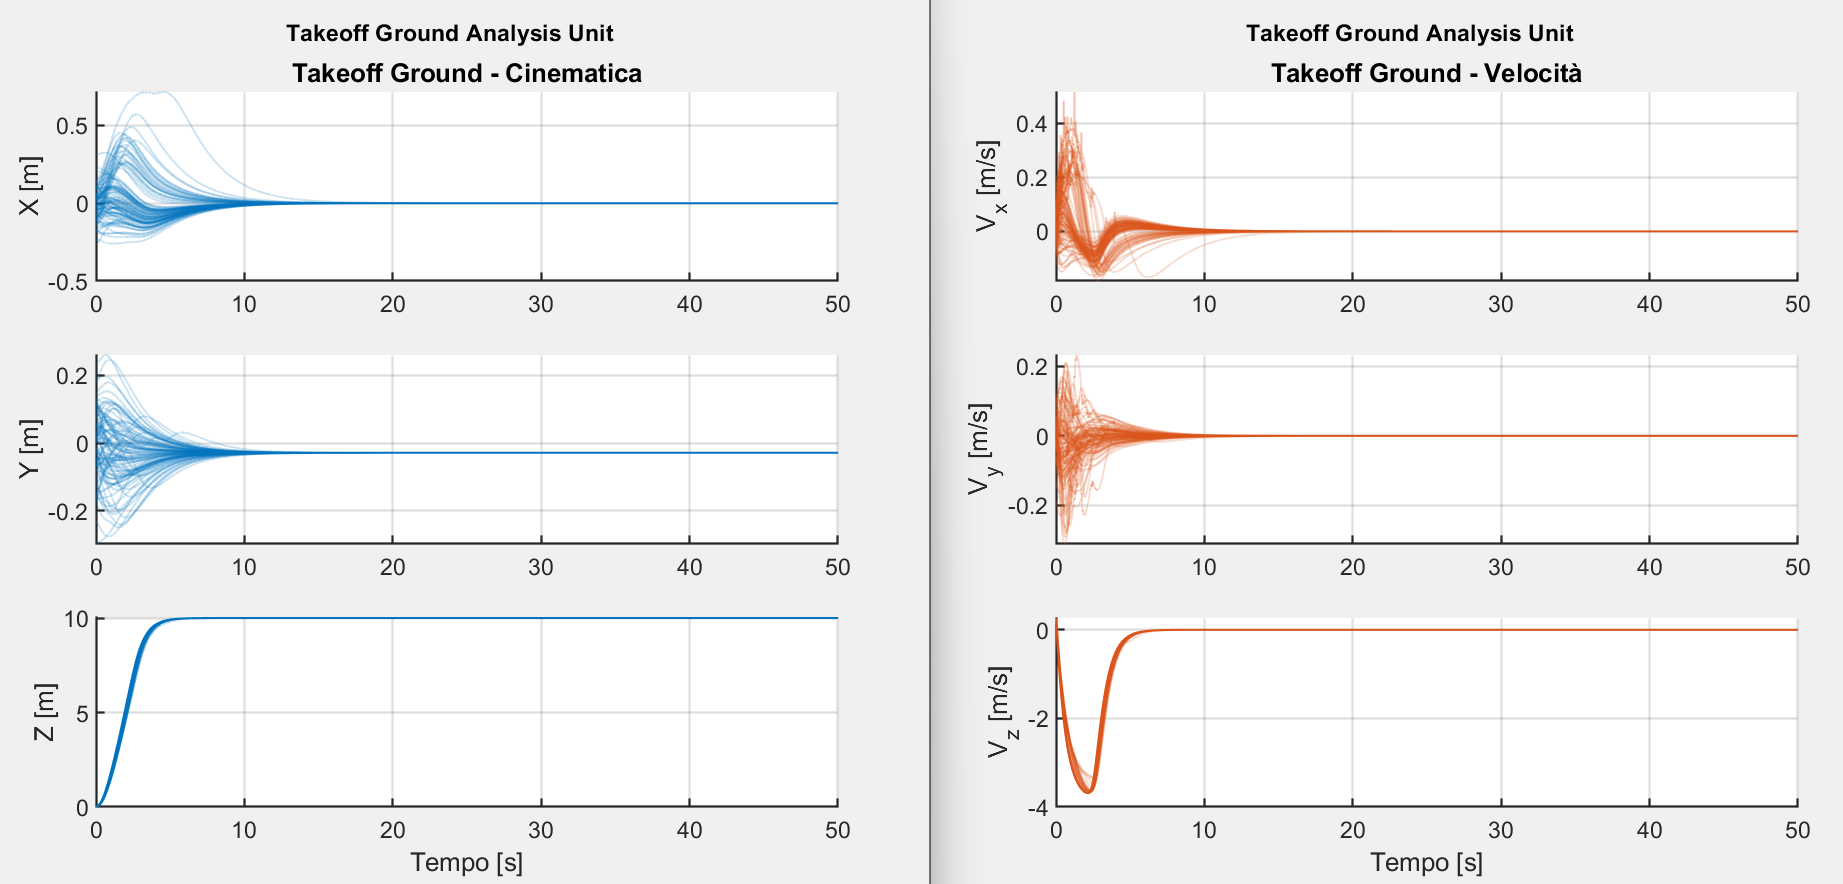
\includegraphics[width=0.8\linewidth]{montecarlo/takeoff_p_v.png}
        \captionof{figure}{Posizione e velocità durante il Takeoff.}
    \end{center}       
\end{frame}

\begin{frame}{Scenario 1: Decollo con SMC}
    \textbf{Obiettivo:} Stabilizzazione dell'assetto.
    \vspace{0.2cm}
    \begin{center}
        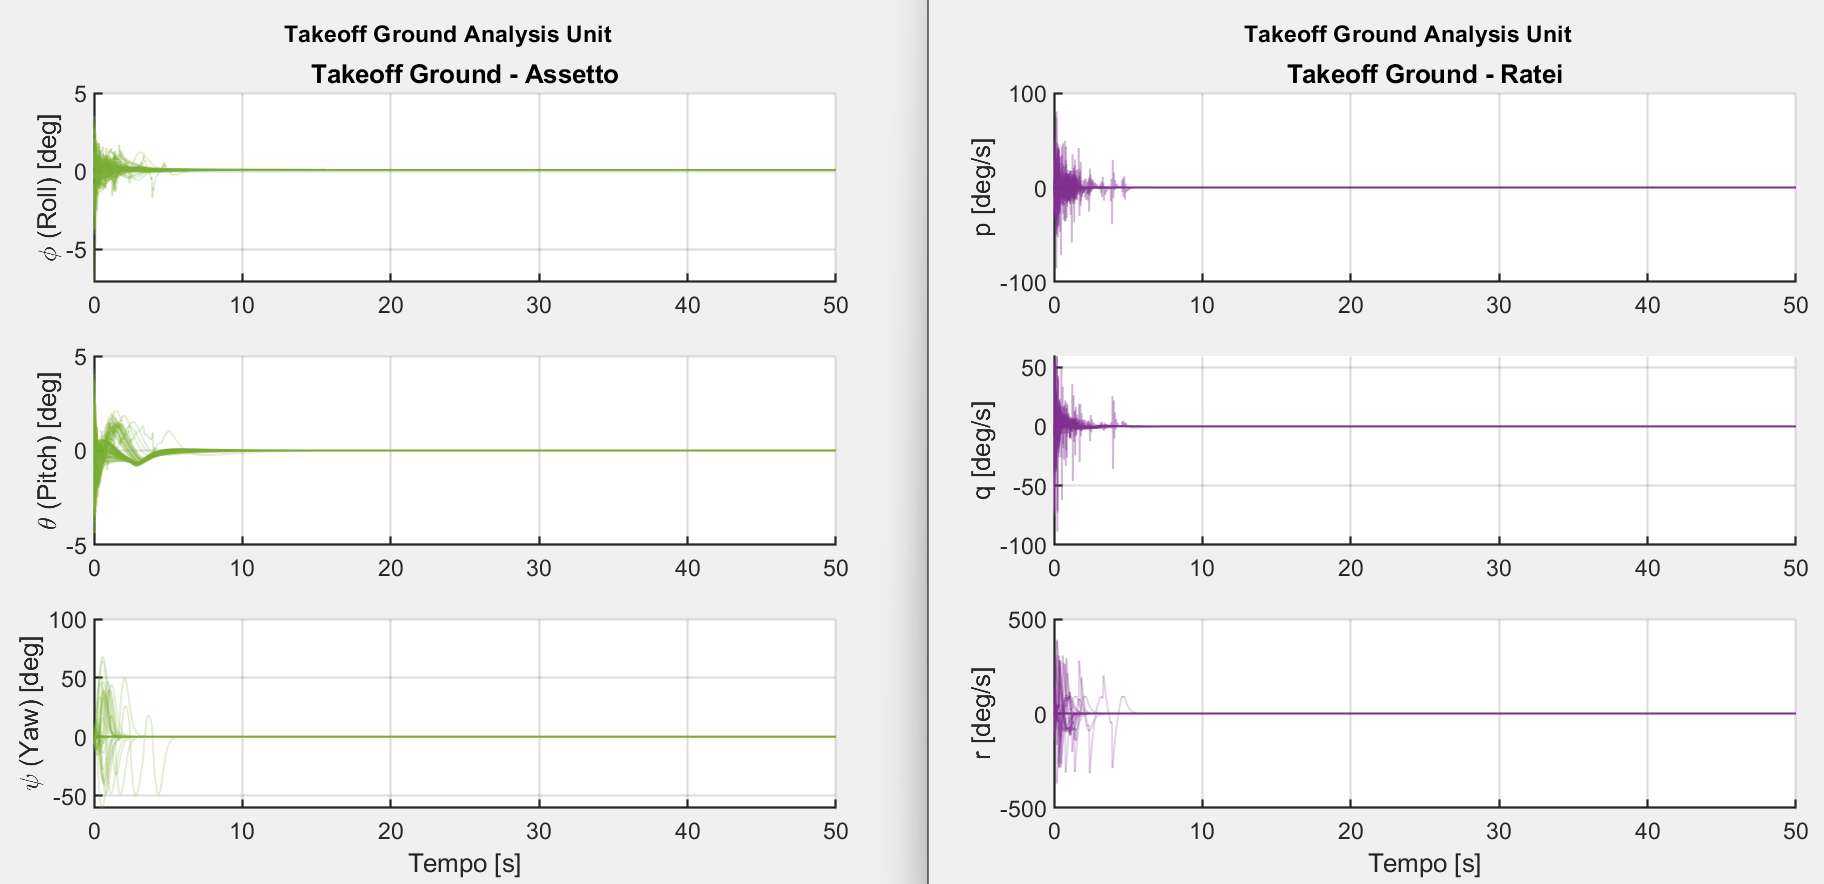
\includegraphics[width=0.8\linewidth]{montecarlo/takeoff_eulero.png}
        \captionof{figure}{Assetto e velocità angolari durante il Takeoff.}
    \end{center}
\end{frame}

% --- SLIDE 3: SMC RECOVERY ---
\begin{frame}{Scenario 2: Recovery con SMC}
    \textbf{Obiettivo:} Mantenimento della posizione e delle velocità.
    \vspace{0.2cm}
    \begin{center}
        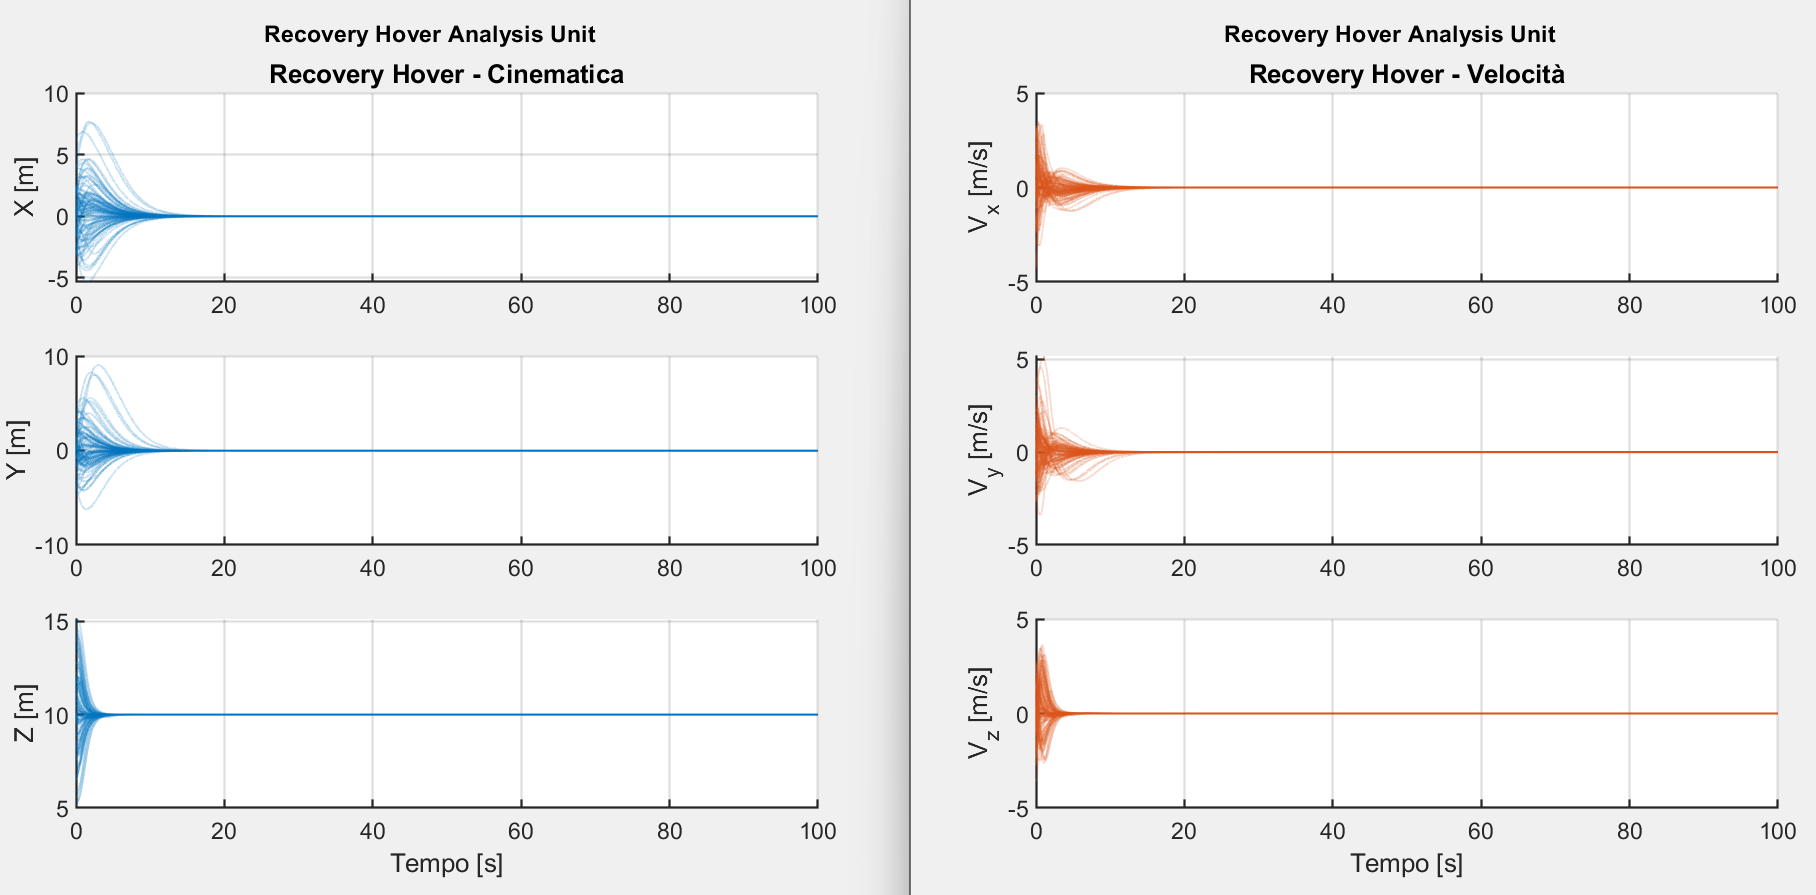
\includegraphics[width=0.8\linewidth]{montecarlo/recovery_p_v.png}
        \captionof{figure}{Posizione e velocità in Hovering.}
    \end{center}  
\end{frame}

\begin{frame}{Scenario 2: Recovery con SMC}
    \textbf{Obiettivo:} Stabilizzazione da assetti estremi ($\pm 15^\circ$).
    \vspace{0.2cm}
    \begin{center}
        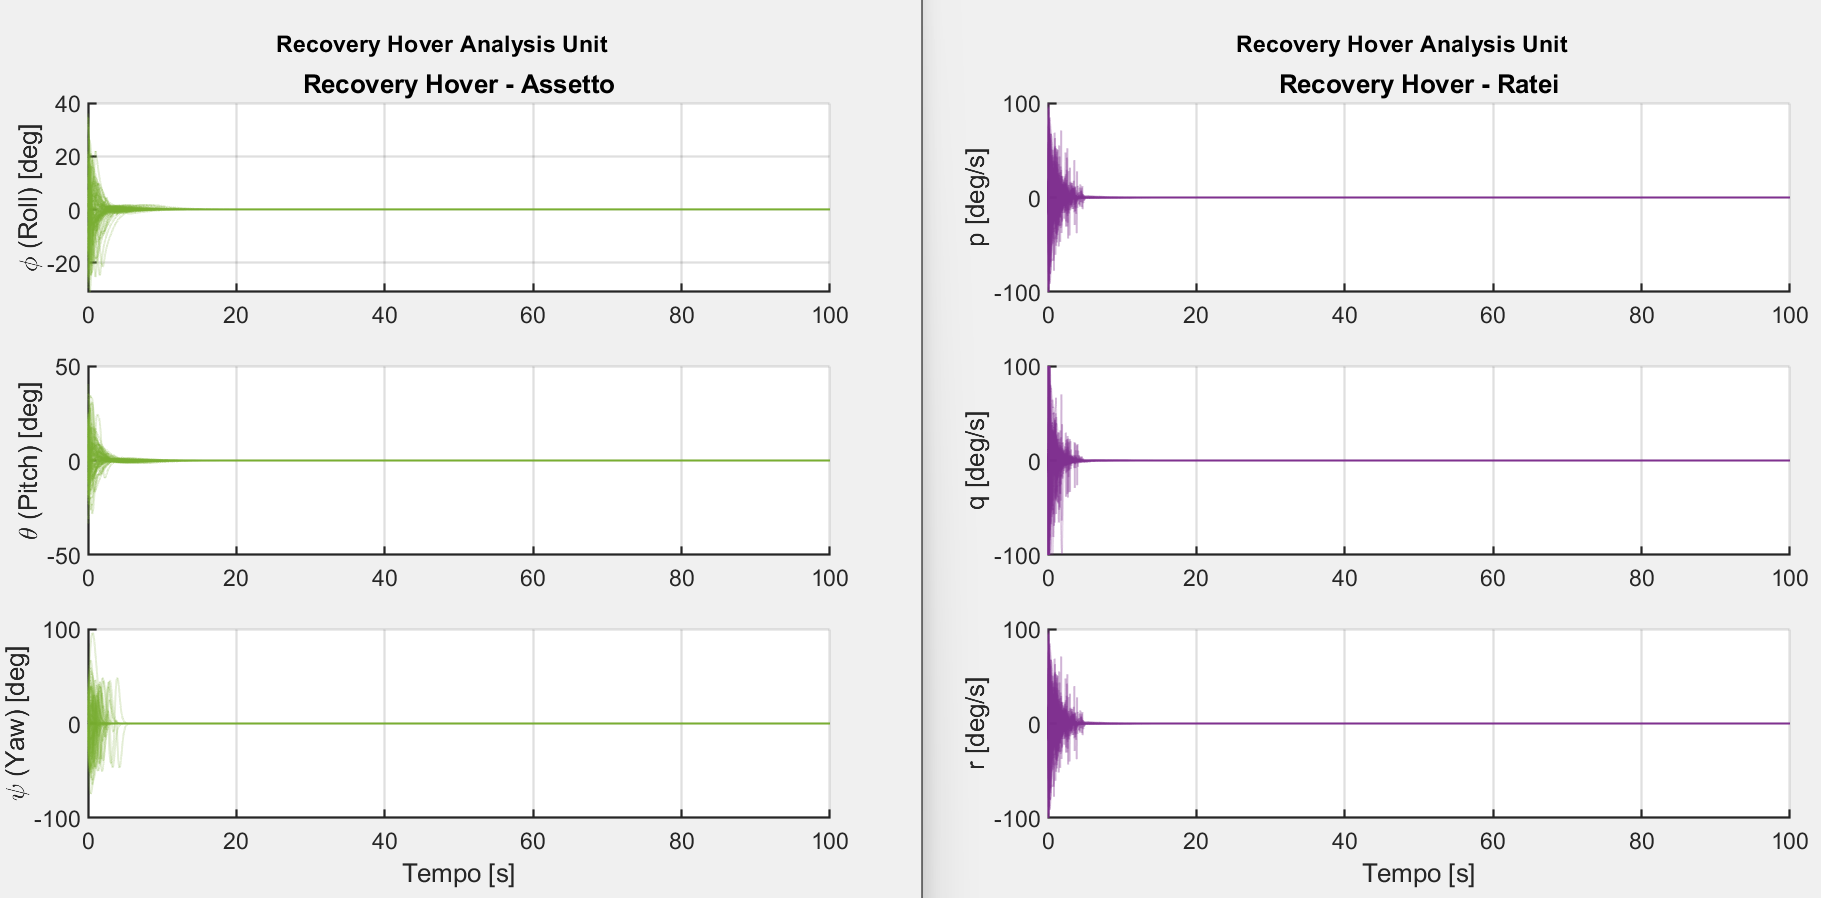
\includegraphics[width=0.8\linewidth]{montecarlo/recovery_eulero.png}
        \captionof{figure}{Assetto e velocità angolari in Hovering.}
    \end{center}  
\end{frame}

% --- SLIDE 4: PID CRUISE ---
\begin{frame}{Scenario 3: Crociera con PID}
    \textbf{Analisi:} Valutazione delle performance del controllo lineare in volo traslato.
    \vspace{0.2cm}
    \begin{center}
        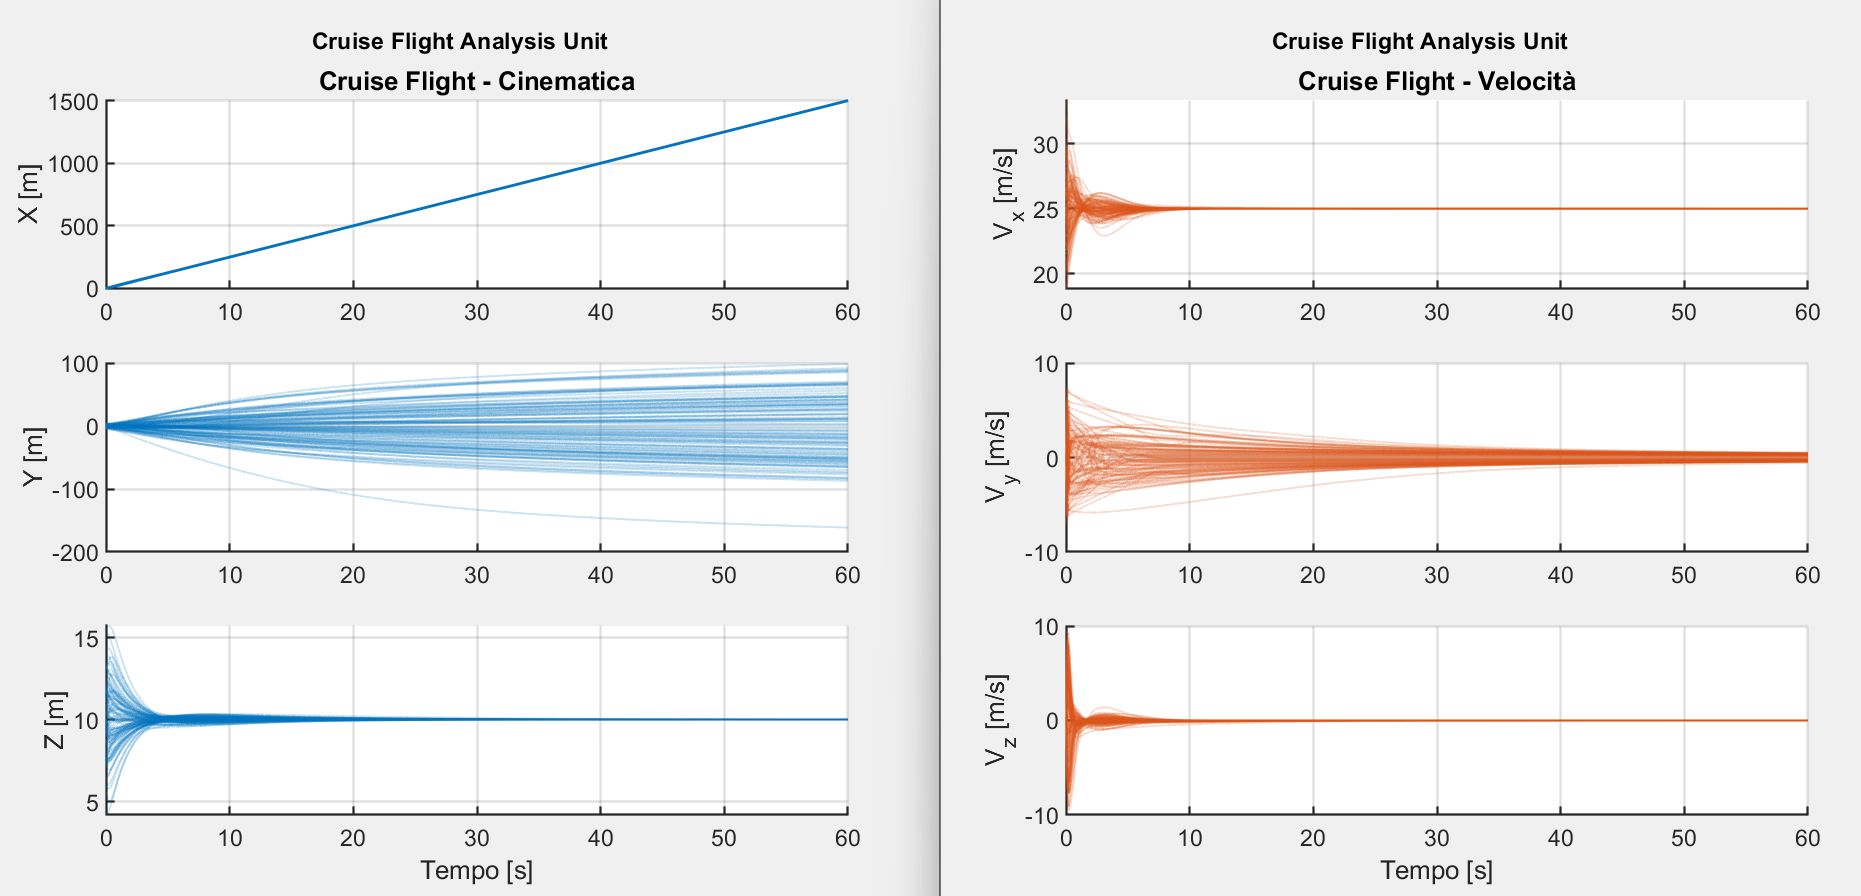
\includegraphics[width=0.8\linewidth]{montecarlo/cruise_p_v.png}
        \captionof{figure}{Posizione e velocità in Crociera.}
    \end{center} 
\end{frame}

\begin{frame}{Scenario 3: Crociera con PID}
    \textbf{Analisi:} Valutazione delle performance del controllo lineare in volo traslato.
    \vspace{0.2cm}
    \begin{center}
        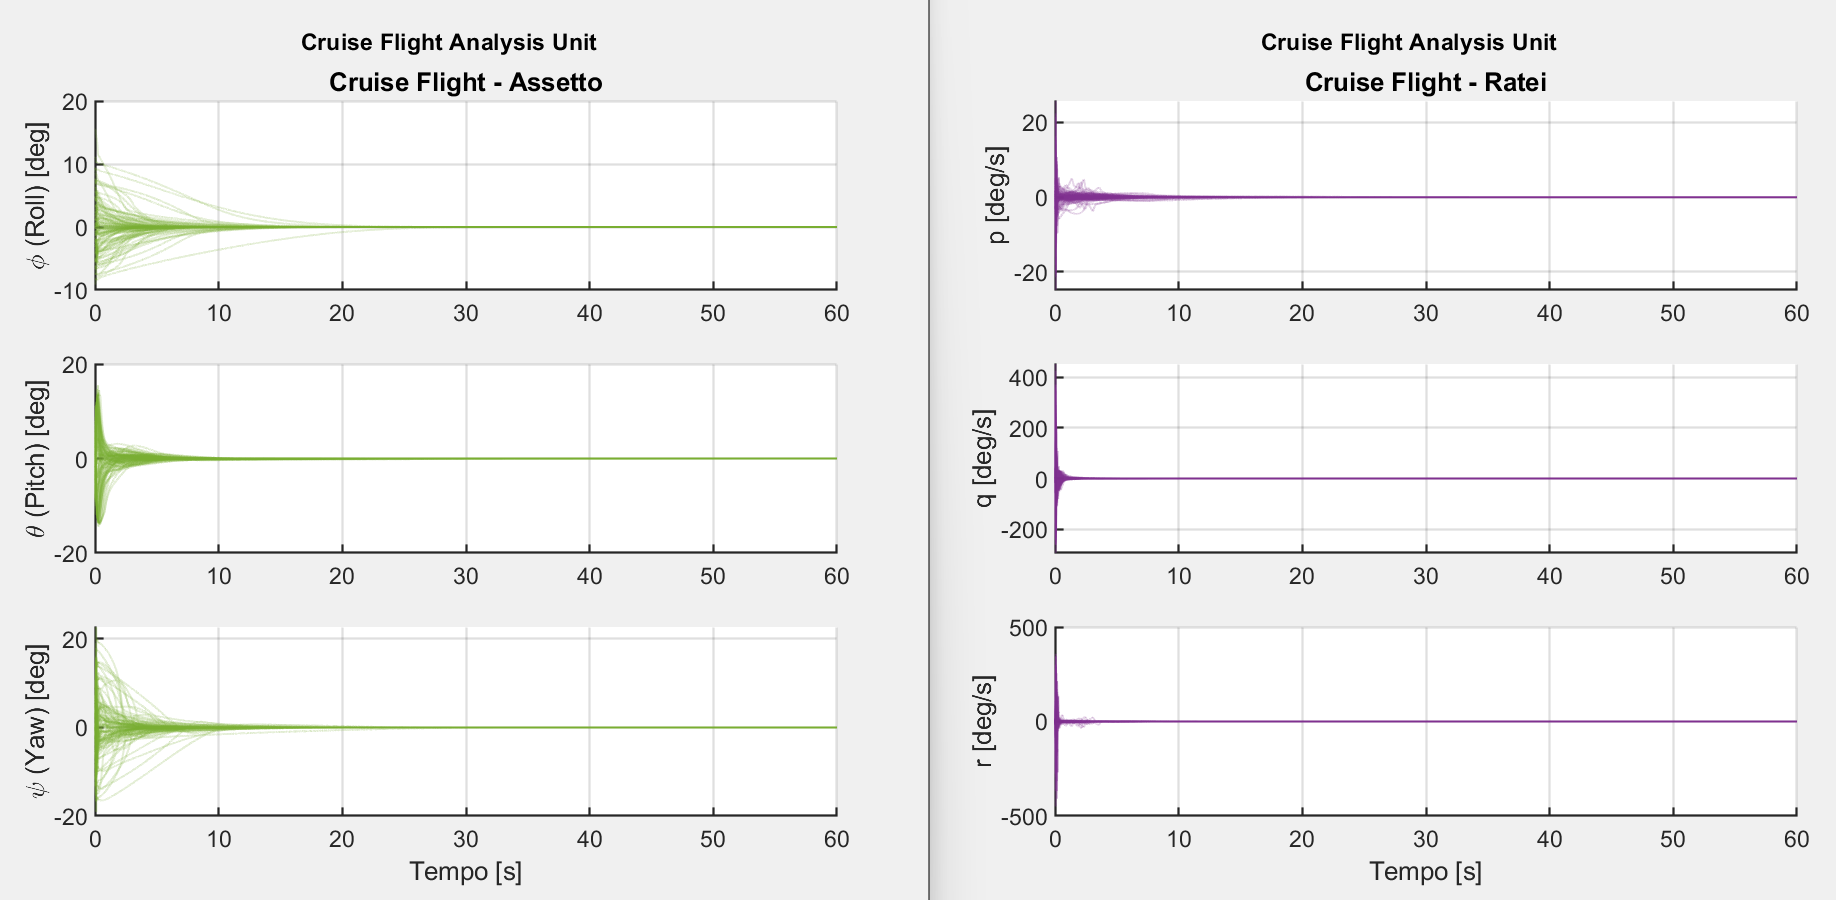
\includegraphics[width=0.8\linewidth]{montecarlo/cruise_eulero.png}
        \captionof{figure}{Assetto e velocità angolari in Crociera.}
    \end{center} 
\end{frame}

% ============================================================
% 5. CONCLUSIONI
% ============================================================
\section{Conclusioni}

\begin{frame}
    \vfill
    \centering
    {\Huge \textbf{Conclusioni}}
    \vfill
\end{frame}

\begin{frame}{Conclusioni e Sviluppi Futuri}
    \textbf{Risultati ottenuti:}
    \begin{itemize}
        \item Modellazione completa a 6-DOF per tricottero tilting-rotor.
        \item Sintesi controllore per il volo verticale.
        \item Sintesi controllore per il volo orizzontale.
    \end{itemize}
    
    \vspace{0.8cm}
    \textbf{Sviluppi Futuri:}
    \begin{itemize}
        \item Sviluppo del controllo laterale per la fase di crociera. 
        \item Analisi di stabilità.
    \end{itemize}
\end{frame}

% \begin{frame}
%     \centering
%     \Huge \textbf{Grazie per l'attenzione}
    
%     \vspace{1cm}
%     \Large Domande?
% \end{frame}

\end{document}
